\documentclass[aspectratio=169,compress]{beamer}
\usepackage[T1]{fontenc}
\usepackage{lmodern,graphicx,xcolor,listings,amssymb,etoolbox}
\definecolor{NordBody}{HTML}{4C566A}
\definecolor{NordBlue}{HTML}{5E81AC}
\definecolor{NordRed}{HTML}{BF616A}
\definecolor{NordPurple}{HTML}{B48EAD}
\definecolor{NordPanel}{HTML}{ECEFF4}
% Retain the custom FRIDA styling while adding Beamer's standard mini-frame
% section navigation.  Completed and current frames are filled; future frames
% remain hollow.  The cumulative-fill state follows the established etoolbox
% approach documented at https://tex.stackexchange.com/questions/61241/.
\useoutertheme[subsection=false]{miniframes}
\setbeamercolor{section in head/foot}{fg=NordBlue,bg=white}
\setbeamercolor{mini frame}{fg=NordBlue,bg=white}
\setbeamercolor{lower separation line head}{bg=NordPanel}
\setbeamerfont{section in head/foot}{size=\tiny}

\newif\ifnavbeforecurrent
\pretocmd\insertnavigation{\navbeforecurrenttrue}{}{}

\newcommand{\fridanavigationdot}{%
  \begin{pgfpicture}{0pt}{0pt}{0.1cm}{0.1cm}
    \pgfpathcircle{\pgfpoint{0.05cm}{0.05cm}}{0.05cm}
    \ifnavbeforecurrent
      \pgfusepath{fill,stroke}
    \else
      \pgfusepath{stroke}
    \fi
  \end{pgfpicture}%
}

\defbeamertemplate*{mini frame}{frida progress}{%
  \begin{pgfpicture}{0pt}{0pt}{0.1cm}{0.1cm}
    \pgfpathcircle{\pgfpoint{0.05cm}{0.05cm}}{0.05cm}
    \pgfusepath{fill,stroke}
  \end{pgfpicture}%
  \global\navbeforecurrentfalse
}
\defbeamertemplate*{mini frame in current section}{frida progress}{\fridanavigationdot}
\defbeamertemplate*{mini frame in current subsection}{frida progress}{\fridanavigationdot}
\defbeamertemplate*{mini frame in other section}{frida progress}{\fridanavigationdot}
\defbeamertemplate*{mini frame in other subsection}{frida progress}{\fridanavigationdot}
\setbeamertemplate{mini frame}[frida progress]
\setbeamertemplate{mini frame in current section}[frida progress]
\setbeamertemplate{mini frame in current subsection}[frida progress]
\setbeamertemplate{mini frame in other section}[frida progress]
\setbeamertemplate{mini frame in other subsection}[frida progress]

\newcommand{\framesource}{}
\BeforeBeginEnvironment{frame}{\gdef\framesource{}}
\newcommand{\slidesource}[1]{\gdef\framesource{#1}}
\setbeamertemplate{footline}{%
  \hbox{%
    \begin{beamercolorbox}[wd=.12\paperwidth,ht=2.7ex,dp=1.2ex,leftskip=1em]{page number in head/foot}%
      \usebeamerfont{page number in head/foot}\insertframenumber\,/\,\inserttotalframenumber
    \end{beamercolorbox}%
    \begin{beamercolorbox}[wd=.88\paperwidth,ht=2.7ex,dp=1.2ex,rightskip=1em plus 1fil]{normal text}%
      \fontsize{5.5}{6.5}\selectfont\framesource
    \end{beamercolorbox}%
  }%
}
\beamertemplatenavigationsymbolsempty
\setbeamercolor{normal text}{fg=NordBody}
\setbeamercolor{title}{fg=NordBlue}
\setbeamercolor{frametitle}{fg=NordBlue}
\setbeamercolor{structure}{fg=NordBlue}
\hypersetup{colorlinks=true,allcolors=NordBlue}
\setbeameroption{hide notes}
\lstset{basicstyle=\ttfamily\fontsize{10}{13}\selectfont\color{NordBody},keywordstyle=\color{NordBlue},commentstyle=\color{NordPurple},columns=fullflexible,keepspaces=true,showstringspaces=false,aboveskip=0pt,belowskip=0pt}
\title{Background}
\author{Kennedy Caisley}
\institute{University of Bonn}
\date{Hotpot workshop}
\newcommand{\checkitem}[2]{\item[$\square$] \textcolor{NordBlue}{#1}\\[2pt]{\normalsize #2}}
\begin{document}
\section{Overview}
\begin{frame}{What we want to build}
\slidesource{\href{https://commons.wikimedia.org/wiki/File:NXP_PCF8577C_LCD_driver_with_I\%C2\%B2C_(Colour_Corrected).jpg}{Die photo: Wikimedia Commons}}
\begin{columns}[c,onlytextwidth]
\begin{column}{.54\textwidth}\centering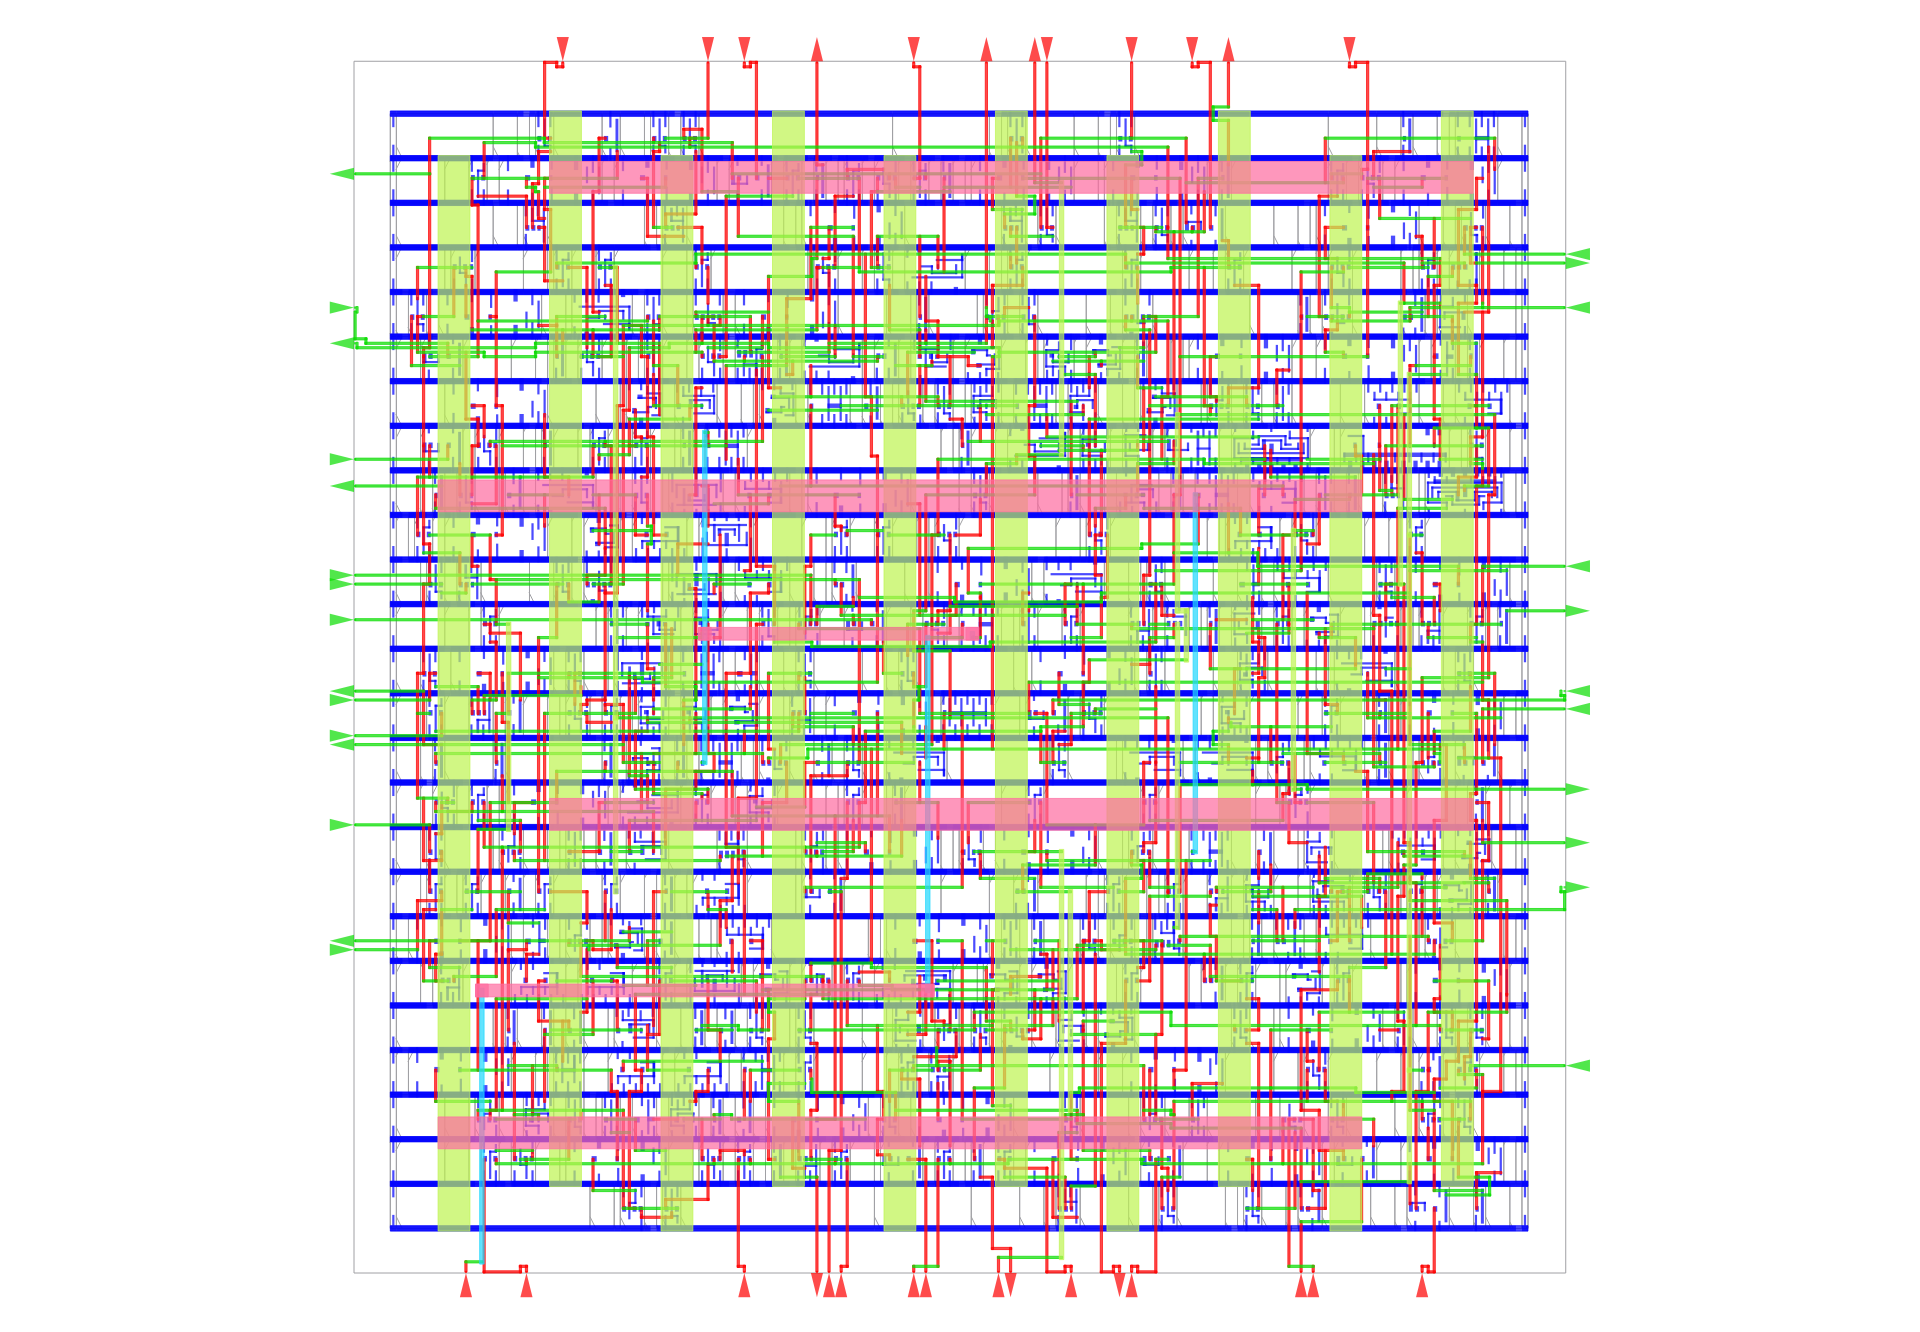
\includegraphics[width=\linewidth,height=.72\textheight,keepaspectratio]{../../images/design.png}\\[4pt]{\small Our GCD layout: Nangate45}\end{column}
\begin{column}{.43\textwidth}\centering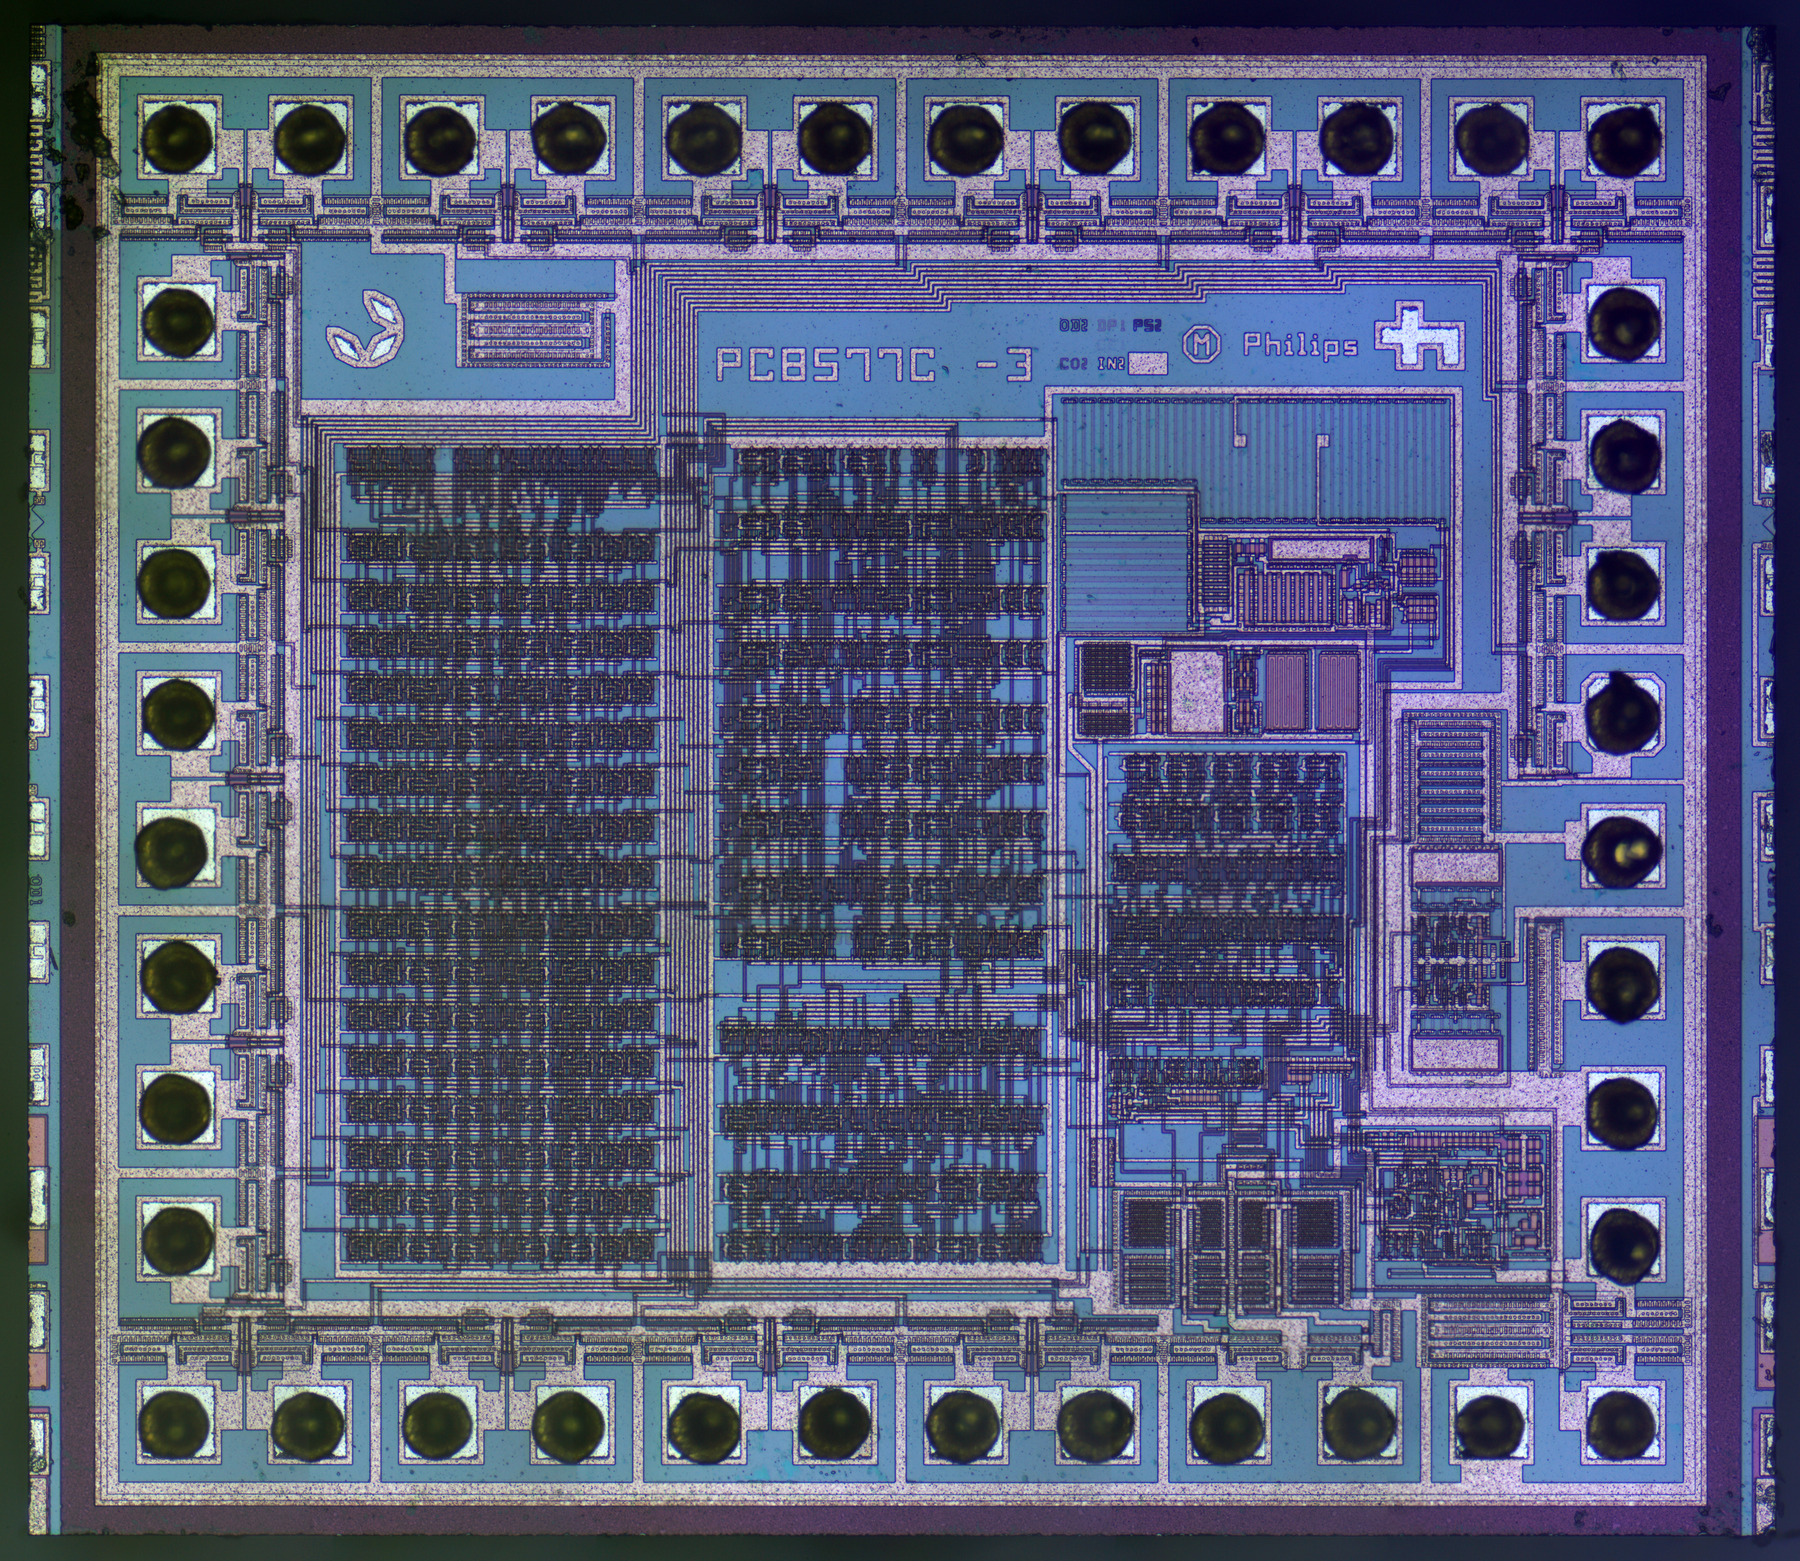
\includegraphics[width=\linewidth,height=.72\textheight,keepaspectratio]{assets/nxp-die-slide.jpg}\\[4pt]{\small A fabricated IC: NXP LCD driver}\end{column}
\end{columns}
\note{The right photograph is an example of manufactured silicon, not the GCD design or Nangate45 process. Photo: cole8888 (Cole L), CC BY-SA 2.0, resized and recompressed. Full source and license: research/SOURCES.md.}
\end{frame}
\begin{frame}{What do we need to build a digital ASIC design?}
\slidesource{\href{https://github.com/The-OpenROAD-Project/OpenROAD}{OpenROAD flow}}
\begin{columns}[c,onlytextwidth]
\begin{column}{.70\textwidth}
{\large\textcolor{NordBlue}{A library of standard cells}}\\[3pt]
Primitive circuit blocks\\[22pt]
{\large\textcolor{NordBlue}{A library of tools}}\\[3pt]
Edit, connect and analyze the design: OpenROAD\\[22pt]
{\large\textcolor{NordBlue}{A flow}}\\[3pt]
A Tcl or Python script to assemble the design
\end{column}
\begin{column}{.24\textwidth}\centering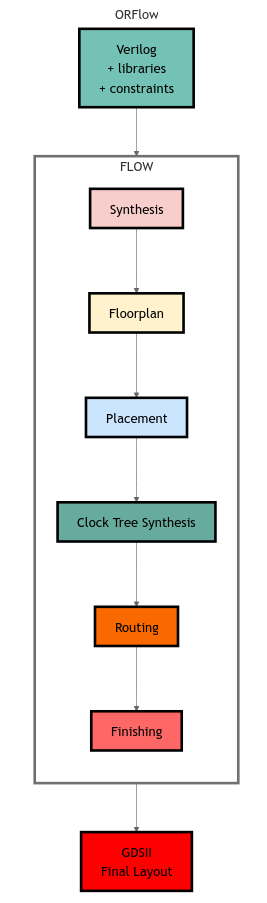
\includegraphics[height=.80\textheight]{assets/openroad-flow.png}\end{column}
\end{columns}
\note{The workshop starts from a synthesized netlist. Technology data, design netlist and constraints are additional concrete inputs. Representations overlap: Verilog also expresses behavior.}
\end{frame}
\begin{frame}{What do we need to build a digital ASIC design?}
\slidesource{\href{https://github.com/The-OpenROAD-Project/OpenROAD}{OpenROAD flow}}
\begin{columns}[c,onlytextwidth]
\begin{column}{.70\textwidth}
{\large\textcolor{NordBlue}{A library of standard cells}}\\[3pt]
Primitive circuit blocks\\[5pt]
{\small Connectivity\quad Physical\quad Logic, timing and power}\\[17pt]
{\large\textcolor{NordBlue}{A library of tools}}\\[3pt]
Edit, connect and analyze the design: OpenROAD\\[22pt]
{\large\textcolor{NordBlue}{A flow}}\\[3pt]
A Tcl or Python script to assemble the design
\end{column}
\begin{column}{.24\textwidth}\centering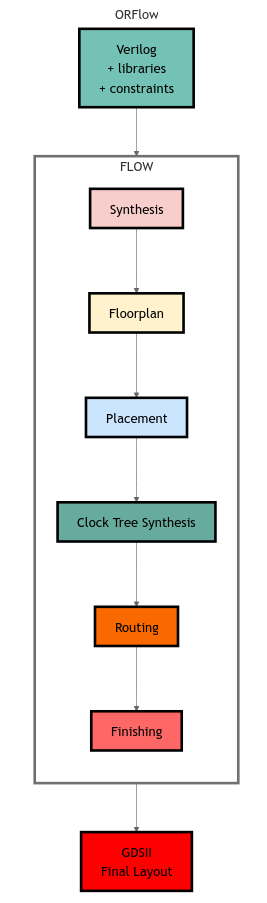
\includegraphics[height=.80\textheight]{assets/openroad-flow.png}\end{column}
\end{columns}
\note{The workshop starts from a synthesized netlist. Technology data, design netlist and constraints are additional concrete inputs. Representations overlap: Verilog also expresses behavior.}
\end{frame}
\begin{frame}{Fabs with open process design kits}
\slidesource{Sources: \href{https://commons.wikimedia.org/wiki/File:SkyWater_Building_Exterior.jpg}{Wikimedia}\enspace\textperiodcentered\enspace\href{https://www.ihp-microelectronics.com}{IHP}\enspace\textperiodcentered\enspace\href{https://gf.com/manufacturing/singapore/}{GlobalFoundries}}
\centering
\includegraphics[width=\textwidth,height=.84\textheight,keepaspectratio]{assets/fabs/fabs-map.pdf}
\note{These are open PDKs for manufactured technologies, unlike the predictive FreePDK45/Nangate45 platform used in our examples. Fabrication access depends on the shuttle or service. SKY130: SkyWater, Bloomington, Minnesota. IHP SG13G2: 130 nm SiGe BiCMOS, Frankfurt (Oder). GF180MCU: GlobalFoundries, Singapore; the photo identifies the Singapore campus, not a verified GF180MCU production building. The legacy PDK interconnect document says FAB3E; do not infer the current building from that historical name. Current fabrication source: https://www.crowdsupply.com/wafer-space/gf180mcu-run-3 . Other sources and image licenses: assets/fabs/SOURCES.md.}
\end{frame}

\section{Connectivity}
\begin{frame}{Inverter: symbol and Verilog}
\begin{columns}[c,onlytextwidth]
\begin{column}{.45\textwidth}\centering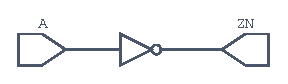
\includegraphics[width=\linewidth]{assets/inverter.pdf}\end{column}
\begin{column}{.49\textwidth}\lstinputlisting[language=Verilog]{examples/inverter.v}\end{column}
\end{columns}
\note{Original ideal functional model. Ports A and ZN agree with the symbol. The assign statement specifies Boolean behavior, not transistor connectivity. The symbol comes from netlistsvg's digital skin, recolored with the Nord palette. https://github.com/nturley/netlistsvg . Uses the Nangate45 INV_X1 cell and pin names.}
\end{frame}
\begin{frame}{SPICE: a circuit becomes an experiment}
\slidesource{\href{https://en.wikipedia.org/wiki/SPICE}{SPICE: Wikipedia}}
\begin{columns}[c,onlytextwidth]\begin{column}{.48\textwidth}\centering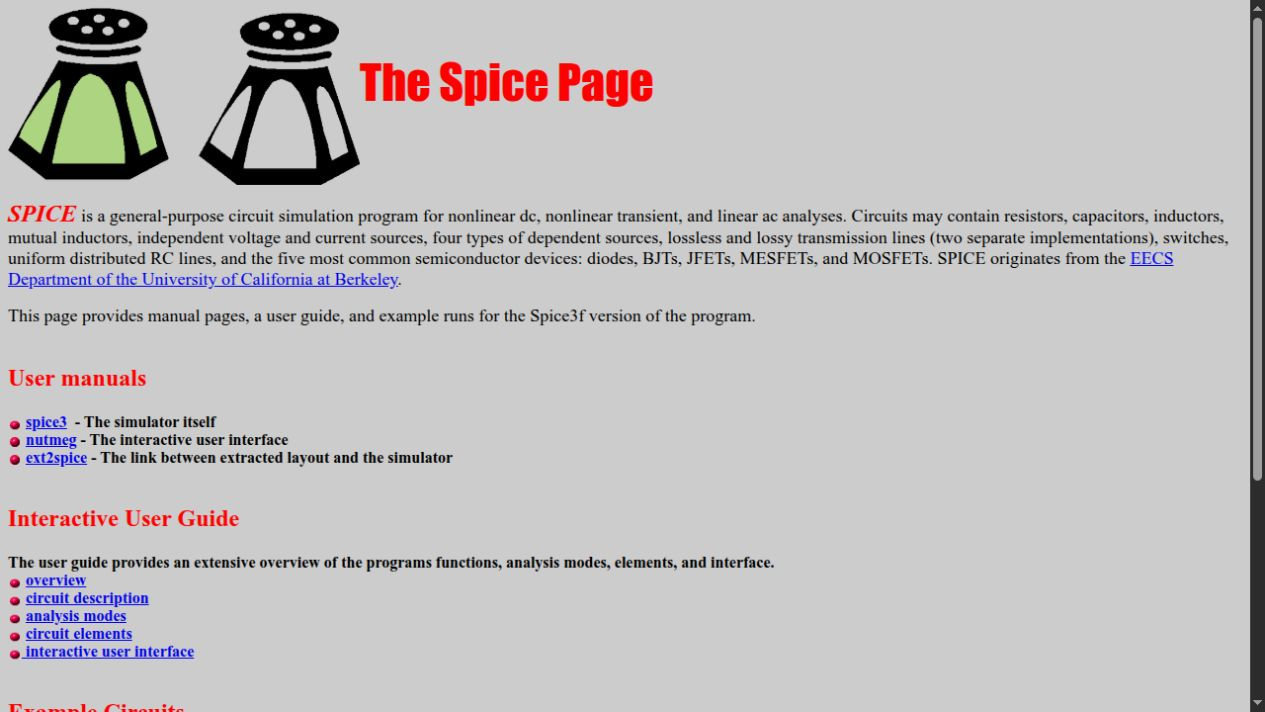
\includegraphics[width=\linewidth,height=.73\textheight,keepaspectratio]{assets/spice-homepage.png}\end{column}\begin{column}{.48\textwidth}
{\Large\textcolor{NordBlue}{Simulation Program with Integrated Circuit Emphasis}}\\[16pt]UC Berkeley, 1973\\[20pt]{\large Simulate devices and models\\under an applied stimulus}\end{column}\end{columns}
\note{Browser screenshot of the Berkeley SPICE page, https://bwrcs.eecs.berkeley.edu/Classes/IcBook/SPICE/ . Nagel and Pederson introduced SPICE in 1973. Netlist dialects vary between simulators.}
\end{frame}
\begin{frame}{Inverter: transistors and SPICE}
\begin{columns}[c,onlytextwidth]
\begin{column}{.35\textwidth}\centering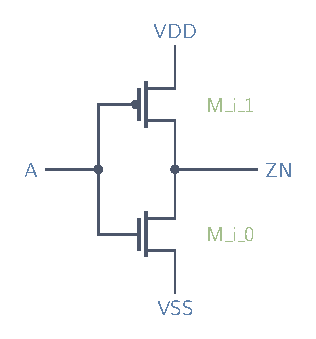
\includegraphics[width=\linewidth,height=.69\textheight,keepaspectratio]{assets/inverter-cmos.pdf}\end{column}
\begin{column}{.62\textwidth}\lstinputlisting[basicstyle=\ttfamily\fontsize{8.8}{11.6}\selectfont\color{NordBody}]{examples/inverter.sp}\end{column}
\end{columns}
\note{Actual INV_X1 excerpt from NangateOpenCellLibrary.cdl, retaining device names, nodes, model names and W/L. Only continuation-line formatting is changed. MOS terminal order is drain, gate, source, bulk. PMOS bulk connects to VDD and NMOS bulk to VSS; bulk connections are explicit in the netlist and implicit in the drawing. This excerpt is not a standalone simulation. Source: https://github.com/The-OpenROAD-Project/OpenROAD-flow-scripts/blob/master/flow/platforms/nangate45/cdl/NangateOpenCellLibrary.cdl .}
\end{frame}
\begin{frame}{NAND: symbol and Verilog}
\begin{columns}[c,onlytextwidth]
\begin{column}{.45\textwidth}\centering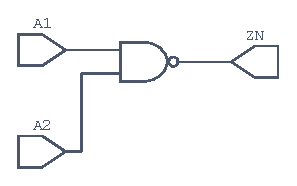
\includegraphics[width=\linewidth]{assets/nand.pdf}\end{column}
\begin{column}{.49\textwidth}\lstinputlisting[language=Verilog]{examples/nand.v}\end{column}
\end{columns}
\note{Original ideal two-input NAND functional model. Uses the Nangate45 NAND2_X1 cell and pins A1, A2 and ZN. Digital symbols: https://github.com/nturley/netlistsvg .}
\end{frame}
\begin{frame}{NAND: transistors and SPICE}
\begin{columns}[c,onlytextwidth]
\begin{column}{.35\textwidth}\centering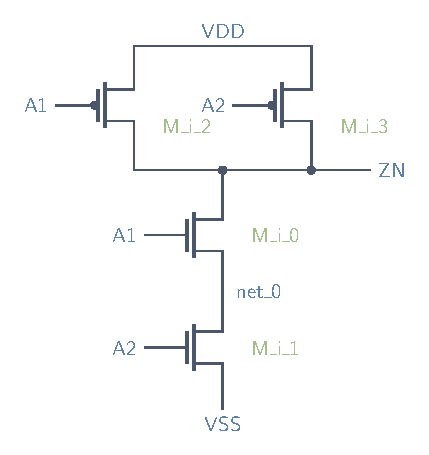
\includegraphics[width=\linewidth,height=.74\textheight,keepaspectratio]{assets/nand-cmos.pdf}\end{column}
\begin{column}{.62\textwidth}\lstinputlisting[basicstyle=\ttfamily\fontsize{8.8}{11.6}\selectfont\color{NordBody}]{examples/nand.sp}\end{column}
\end{columns}
\note{Two parallel PMOS devices pull up; two series NMOS devices pull down. Equal net labels A1 or A2 mean the same connection. net\_0 is the internal series node. Bulk ties are explicit in SPICE and implicit in the drawing. Actual NAND2_X1 excerpt from NangateOpenCellLibrary.cdl, retaining all node, device and model names and dimensions. M\_i\_2 has its drain at VDD and source at ZN as in the original CDL, and is flipped in the drawing to match. Only continuation-line formatting is changed. Source: https://github.com/The-OpenROAD-Project/OpenROAD-flow-scripts/blob/master/flow/platforms/nangate45/cdl/NangateOpenCellLibrary.cdl .}
\end{frame}
\begin{frame}{Connecting cells: the top module}
\begin{columns}[c,onlytextwidth]
\begin{column}{.46\textwidth}\centering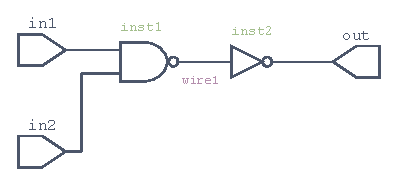
\includegraphics[width=\linewidth]{assets/top.pdf}\end{column}
\begin{column}{.51\textwidth}\lstinputlisting[language=Verilog,basicstyle=\ttfamily\fontsize{8.6}{10.6}\selectfont\color{NordBody}]{examples/top.v}\end{column}
\end{columns}
\note{NAND2\_X1 is the cell/module type and inst1 is one instance. INV\_X1 is the other type and inst2 its instance. Named associations connect each cell port to a net in top. NAND followed by inversion gives out = in1 AND in2. The teaching netlist preserves both cells; logic optimization could change this structure. Original diagram and editable code, inspired by Austin Rovinski's circuit-taxonomy teaching sequence: https://www.youtube.com/watch?v=bRUf6BLq1V0 . No lecture image reused.}
\end{frame}
\begin{frame}{Connectivity: ports, instances and nets}
\centering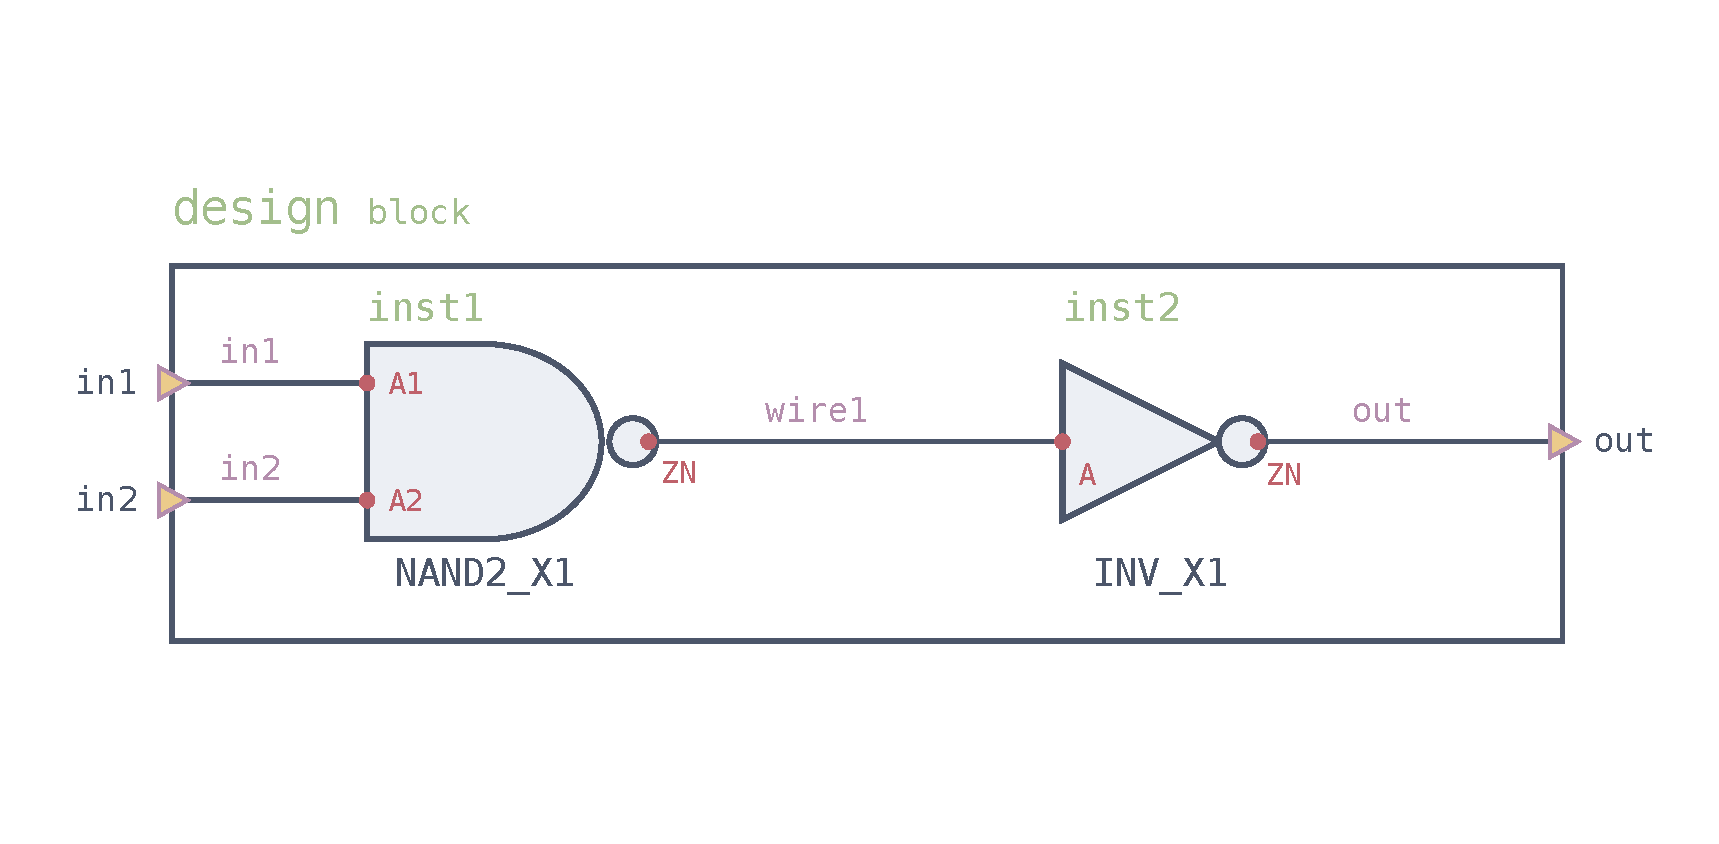
\includegraphics[width=\linewidth,height=.81\textheight,keepaspectratio]{assets/top-detail.pdf}
\note{The same two gate shapes from the generated netlistsvg image, arranged with an explicit top boundary. Green: instance names. Purple: net names. Red: pins on each instance. Boundary markers: ports of top. Each instance has its own terminals even when it shares a cell definition with other instances.}
\end{frame}
\begin{frame}{The same circuit in OpenDB}
\centering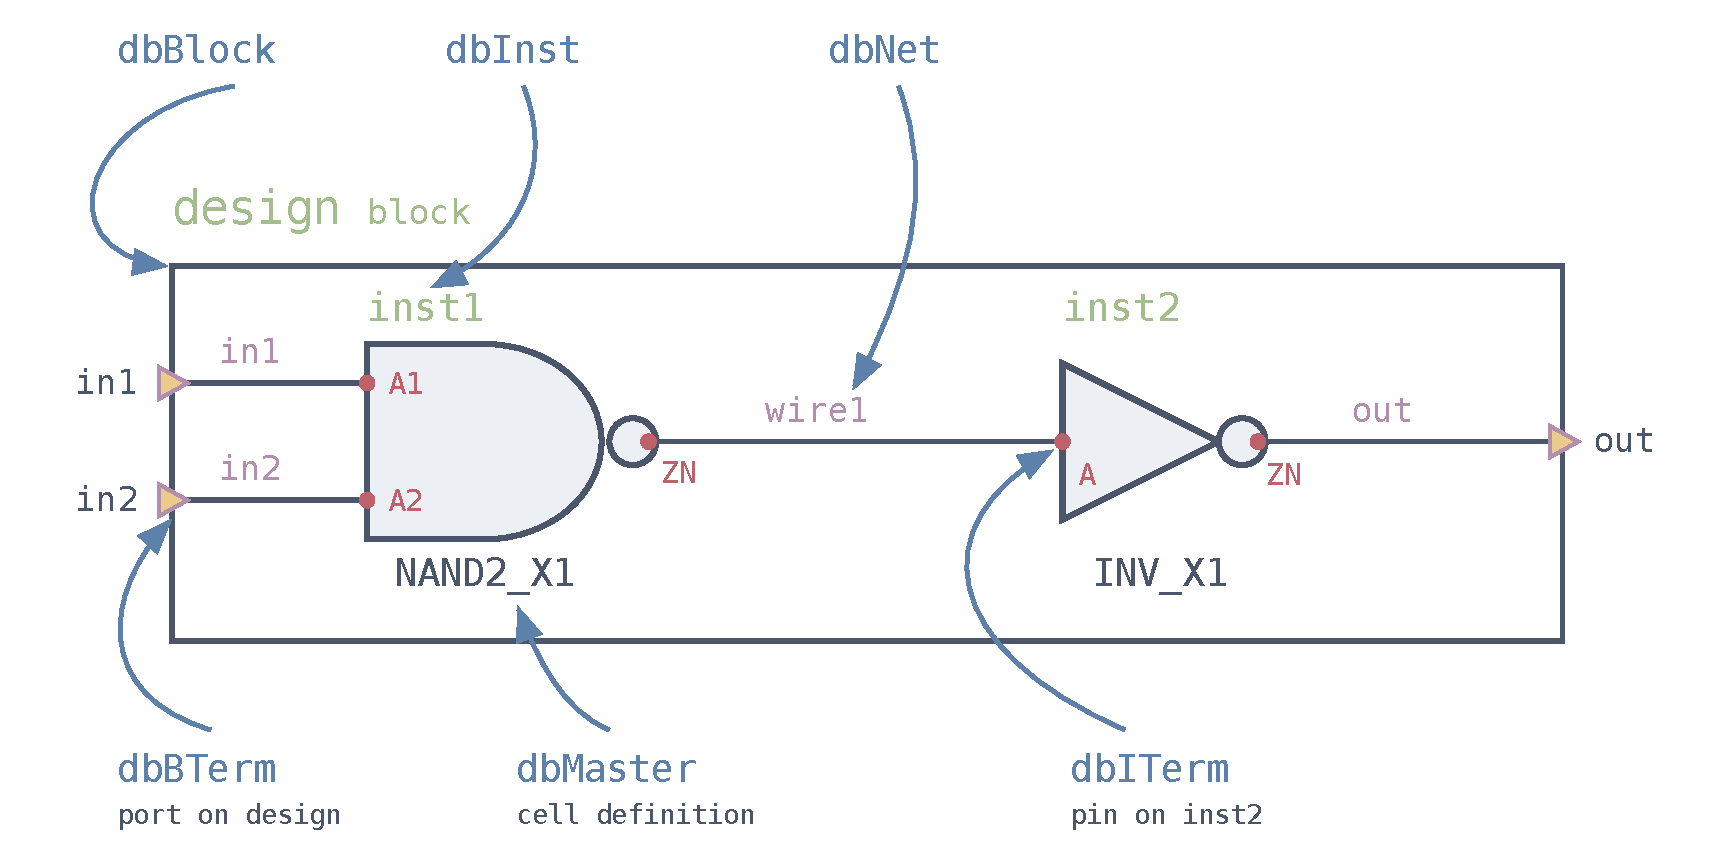
\includegraphics[width=\linewidth,height=.81\textheight,keepaspectratio]{assets/top-opendb.pdf}
\note{dbBlock: top design container. dbBTerm: a terminal at that block's boundary, corresponding here to a top-level port. dbInst: a placed or unplaced use of a library master, here inst1 or inst2. dbITerm: a terminal belonging to that instance. dbNet: connection joining terminals. dbMaster: library cell definition, represented by the NAND2\_X1 type label; it is shared, not owned by one instance. A dbITerm refers to a master terminal (dbMTerm), which defines that library pin. Verilog module definitions and OpenDB masters are related here through library-cell linking, not interchangeable general-purpose objects. Source: https://openroad.readthedocs.io/en/latest/main/src/odb/README.html and OpenROAD src/odb/include/odb/db.h .}
\end{frame}

\section{Physical views}

\begin{frame}{From transistors to bump bonds}
\slidesource{\href{https://commons.wikimedia.org/wiki/File:Cmos-chip_structure_in_2000s_(en).svg}{CMOS stackup image (Source: Wikimedia Commons)}}
\begin{columns}[c,onlytextwidth]
\begin{column}{.49\textwidth}
\centering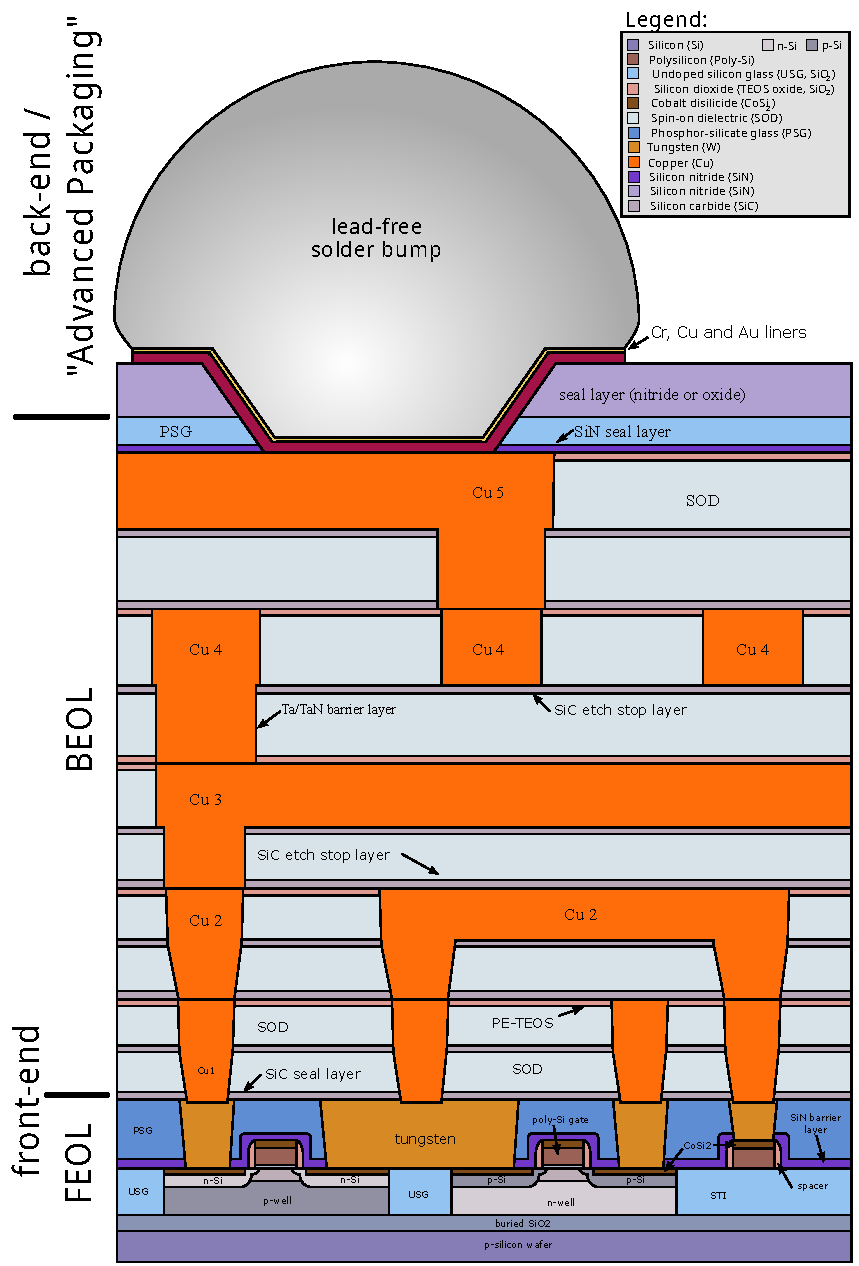
\includegraphics[height=.81\textheight]{assets/cmos-cross-section.pdf}
\end{column}
\begin{column}{.49\textwidth}
\centering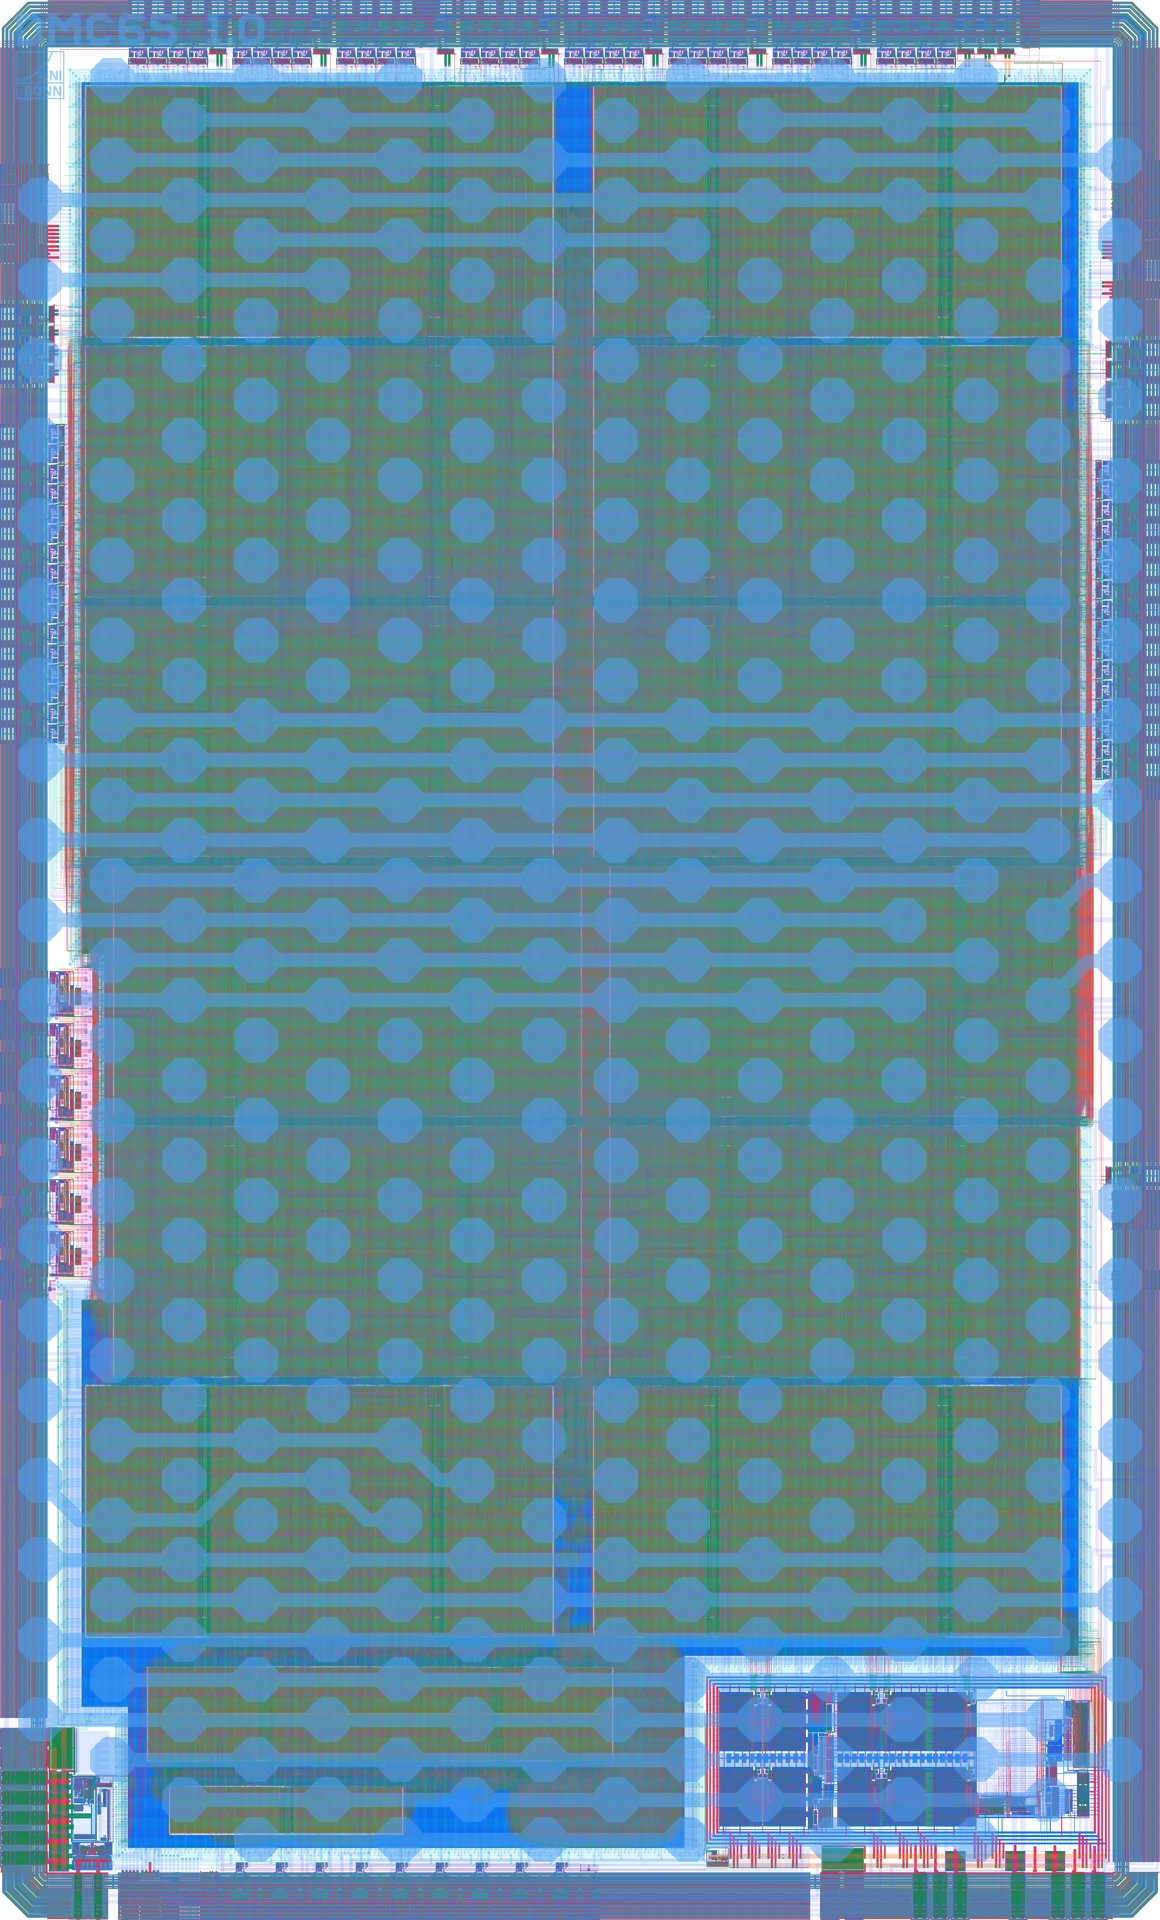
\includegraphics[height=.77\textheight]{assets/dmc65-layout.png}\\[3pt]
{\small\textcolor{NordBlue}{DMC65: bump-pad array}}
\end{column}
\end{columns}
\note{Left: Cmos-chip structure in 2000s (en).svg, Cepheiden (2006), Wikimedia Commons, CC BY-SA 3.0. Original multilingual SVG rendered in English; material legend removed for clarity, then resized and converted to PDF. The adapted illustration retains CC BY-SA 3.0. General early-2000s CMOS-on-SOI illustration with five metallization levels and a flip-chip solder contact; it is not the DMC65 or Nangate45 process cross section. Right: existing local asiclab/projects/dmc65/dmc65_web.webp, copied and losslessly converted to PNG for LaTeX. It is a top-down layout rendering showing bump-pad locations, not a photograph of physical solder bumps. Local provenance identifies DMC65v1/dmc_top/layout revision 4, 13 June 2022, die bounds 2.9 by 4.8 mm; the existing image was produced by the DMC65 ArtistIC workflow.}
\end{frame}

\begin{frame}{GDSII: the mask geometry}
\slidesource{\href{https://en.wikipedia.org/wiki/GDSII}{GDSII: Wikipedia}}
\begin{columns}[c,onlytextwidth]\begin{column}{.48\textwidth}\centering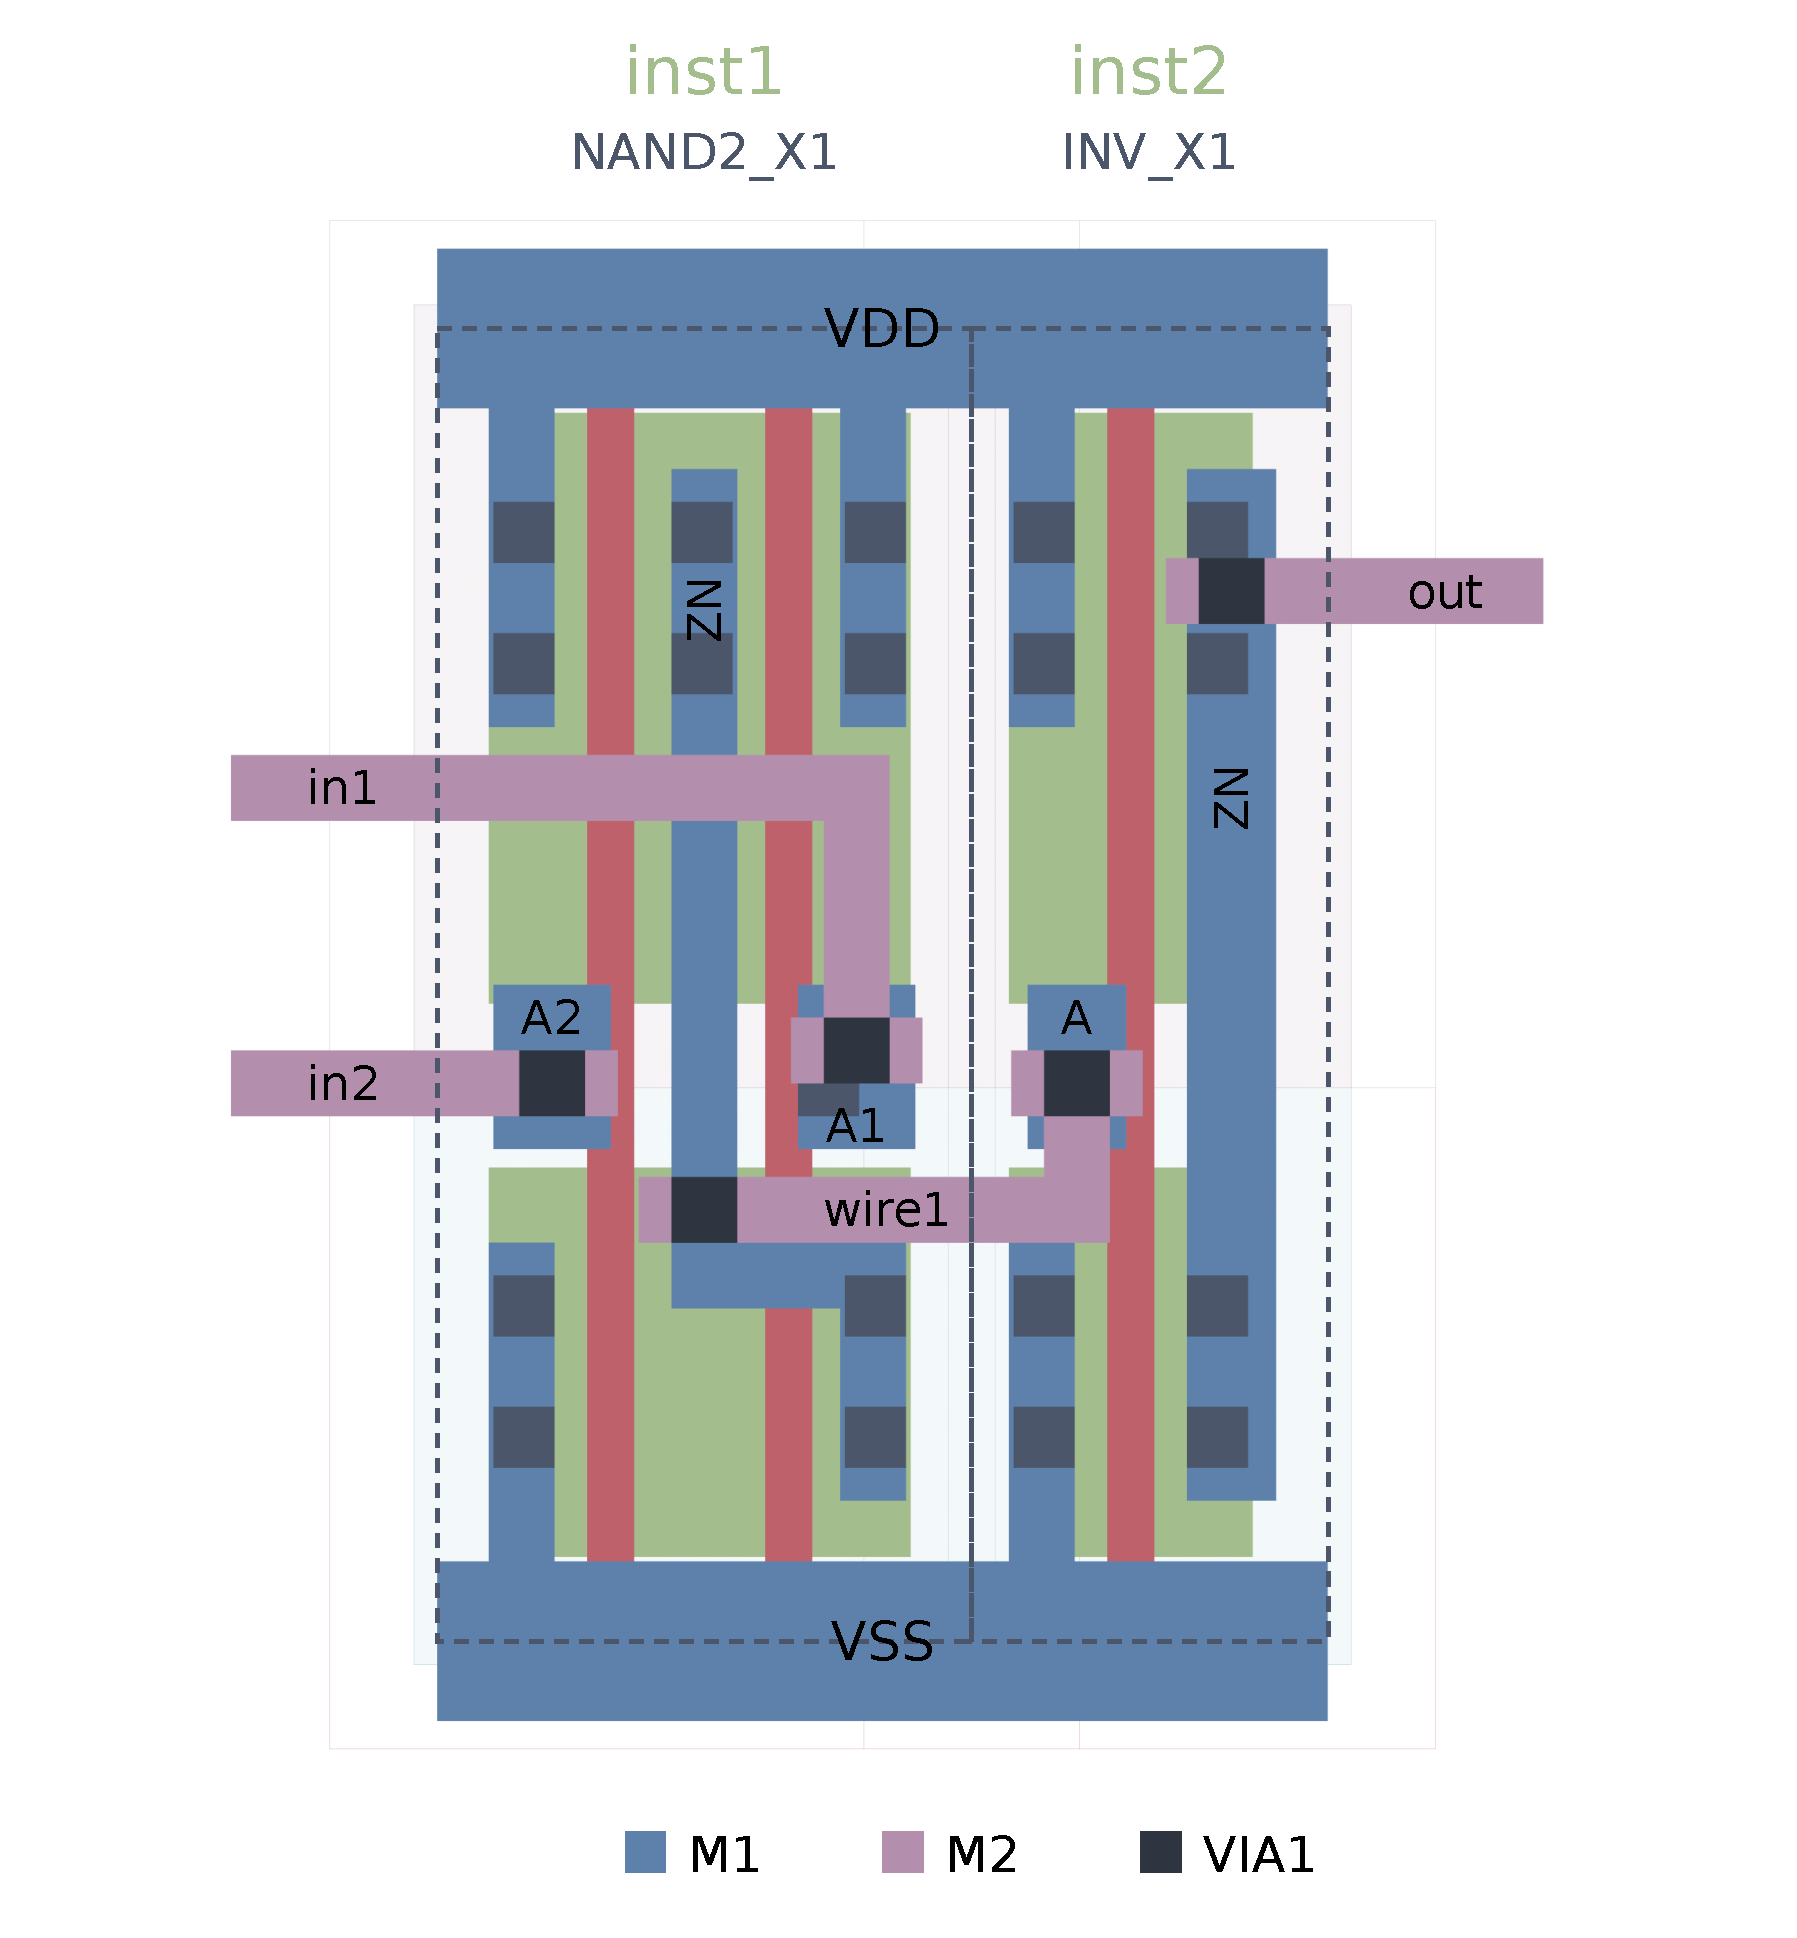
\includegraphics[width=\linewidth,height=.73\textheight,keepaspectratio]{layout/pair_full_labeled.pdf}\end{column}\begin{column}{.48\textwidth}
{\Large\textcolor{NordBlue}{Graphic Design System II}}\\[16pt]Calma, 1978\\[20pt]{\large Hierarchical cells and polygons on numbered layers}\end{column}\end{columns}
\note{Binary stream format, not a text netlist. Historical source: Calma GDS II Users Operating Manual, November 1978, bitsavers.computerhistory.org. Layer meanings come from the technology mapping, not the layer number alone.}
\end{frame}
\begin{frame}{Nangate45: the cell layouts}
\begin{columns}[c,onlytextwidth]
\begin{column}{.49\textwidth}\centering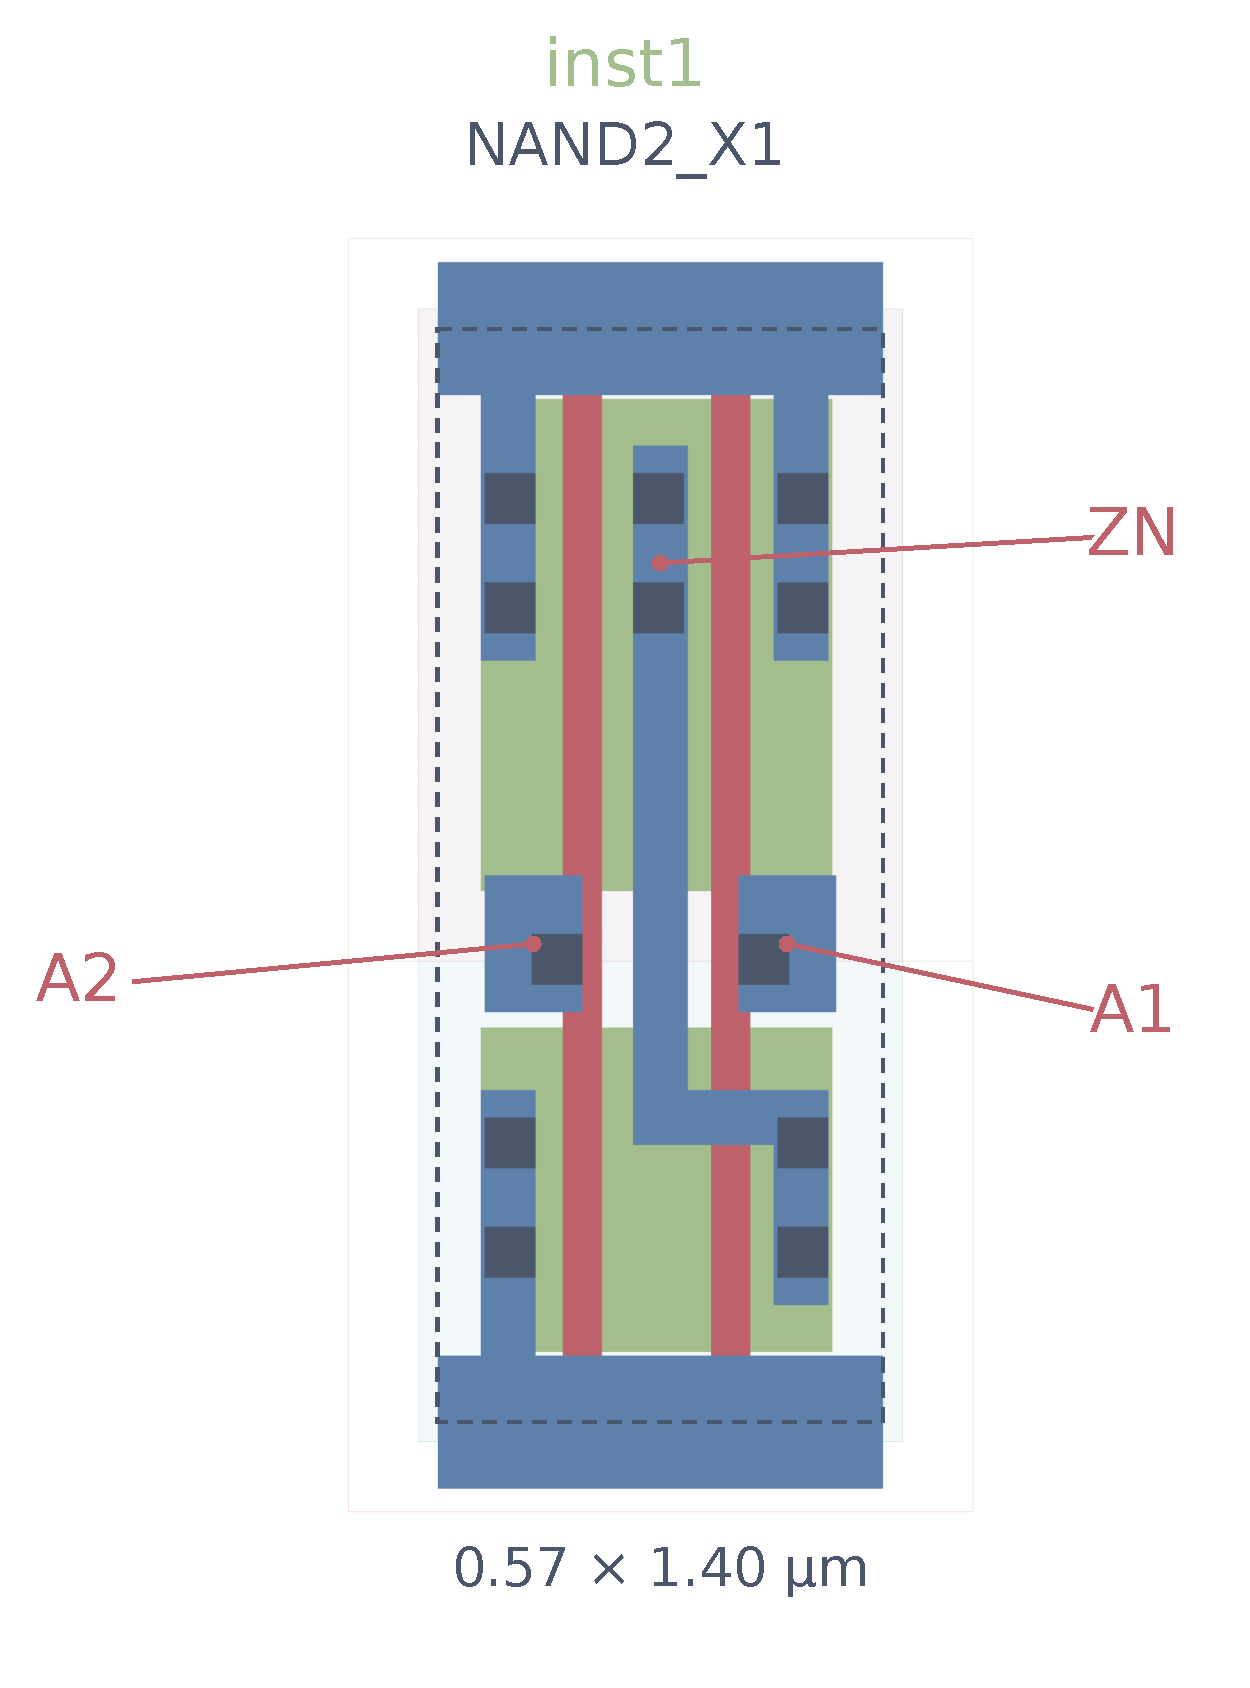
\includegraphics[height=.80\textheight]{layout/nand_cell_labeled.pdf}\end{column}
\begin{column}{.49\textwidth}\centering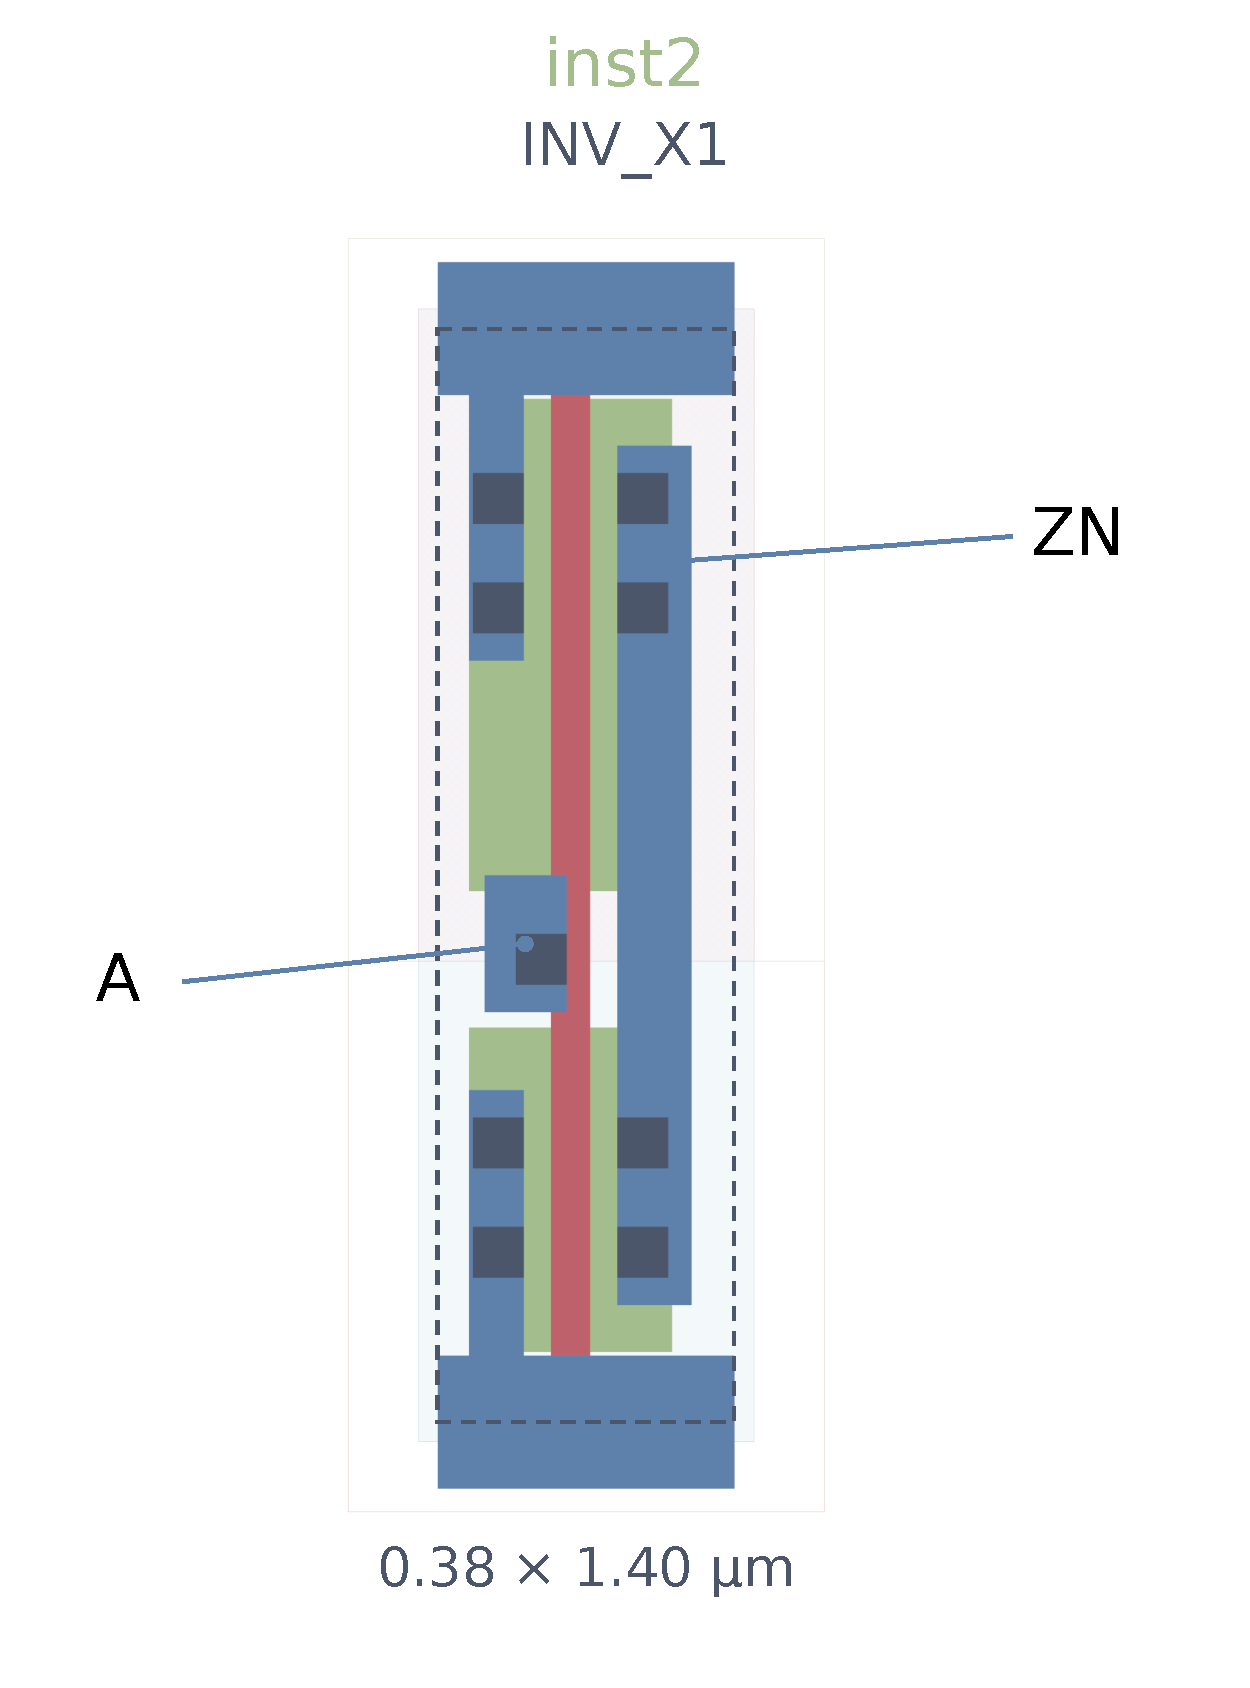
\includegraphics[height=.80\textheight]{layout/inv_cell_labeled.pdf}\end{column}
\end{columns}
\note{Actual NAND2_X1 and INV_X1 GDS layouts from NangateOpenCellLibrary.gds. Pin labels are positioned using the corresponding LEF PORT polygons. These cells have not yet been connected. Instance placement widths are 0.57 and 0.38 micrometers; both are 1.4 micrometers high. Well and implant geometries extend beyond the dashed placement boundaries. Rendered directly with KLayout, using the local Nangate45 Nord layer properties. Sources: https://github.com/The-OpenROAD-Project/OpenROAD-flow-scripts/tree/master/flow/platforms/nangate45 .}
\end{frame}
\begin{frame}{Physical view: connecting the cells}
\centering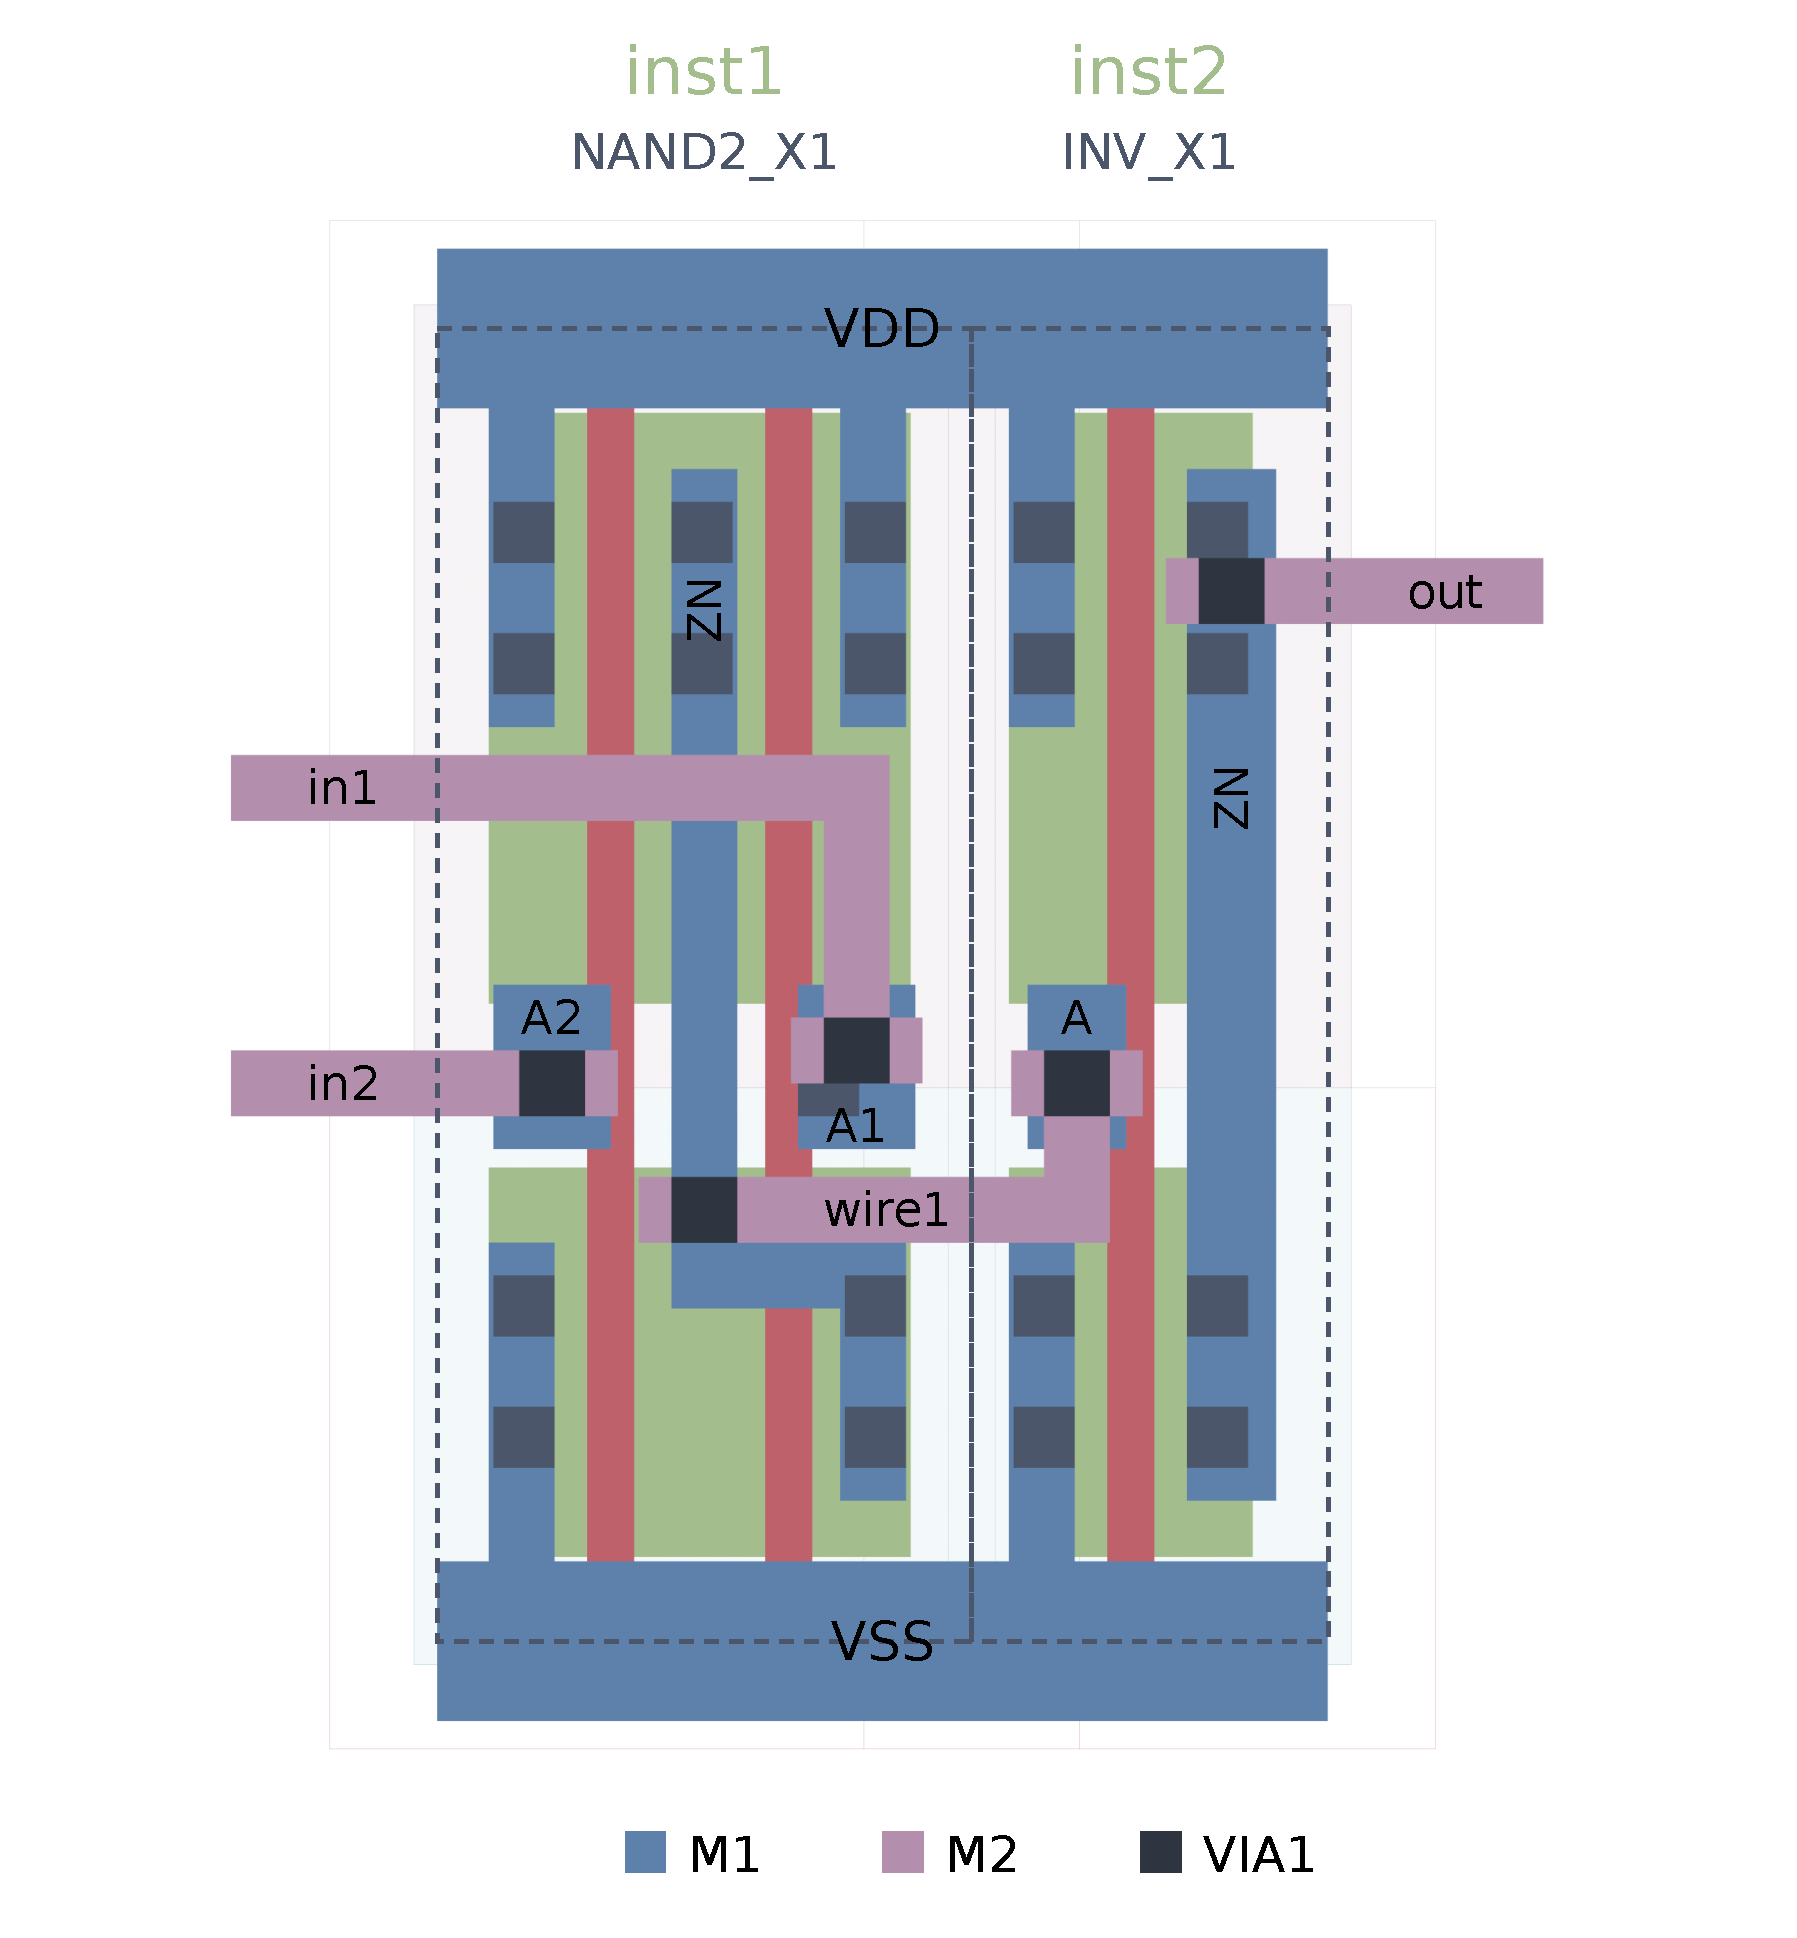
\includegraphics[height=.82\textheight]{layout/pair_full_labeled.pdf}
\note{Original GDS masters abutted without modifying their internal geometry. Manual demonstration M2 routes connect inst1/ZN to inst2/A and extend in1, in2 and out to access points outside the cell pair. VIA1 uses the via1_5 definition from the Nangate45 technology LEF. Adjacent M1 power rails abut. This is a teaching layout, not an OpenROAD-routed or DRC/LVS-signoff result. Via cuts were checked against intended LEF pins and M2 routes checked for shorts. All physical mask layers present in these cells are shown; GDS text and boundary-marker layers are replaced with annotations.}
\end{frame}
\begin{frame}{Physical view: M1, M2 and vias}
\centering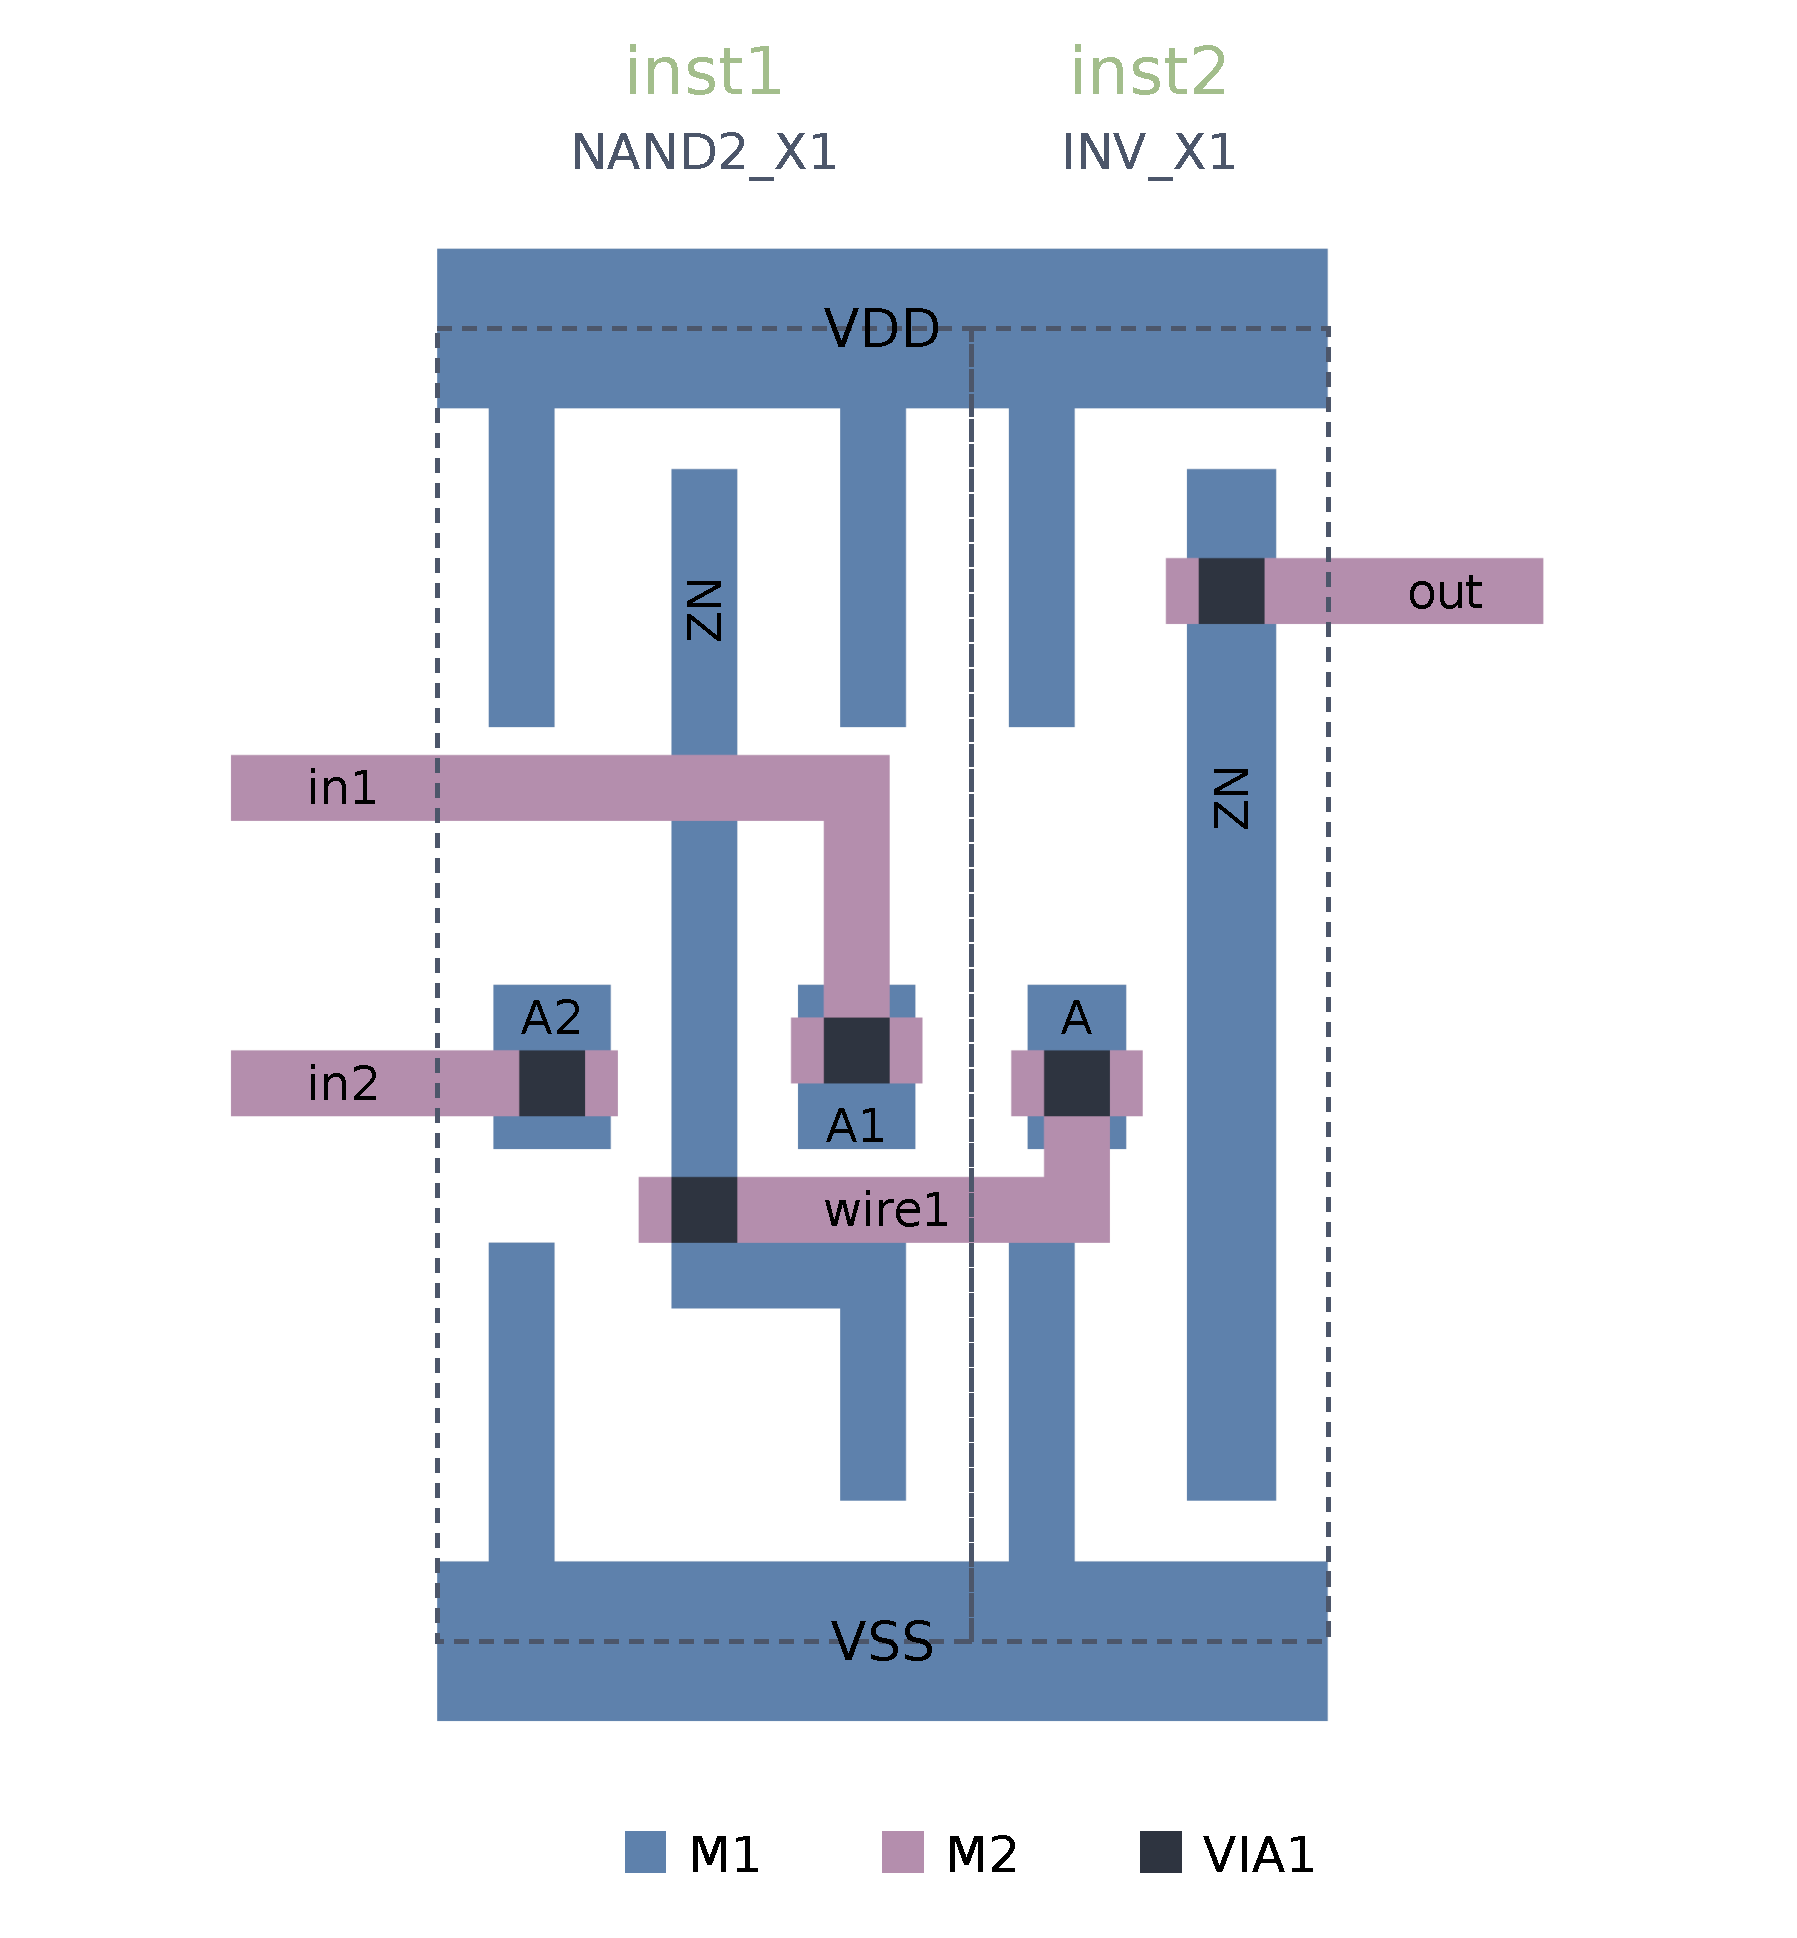
\includegraphics[height=.82\textheight]{layout/pair_metal_labeled.pdf}
\note{Exactly the same connected GDS and framing, with lower layers hidden. Blue is M1, purple is M2, and dark squares are VIA1 cuts. A crossing between M1 and M2 is connected only where there is a via. This is a filtered GDS view, not yet a LEF abstract.}
\end{frame}
\section{LEF}
\begin{frame}{LEF / DEF: the physical design interchange}
\slidesource{\href{https://si2.org/lef-def-downloads/}{Si2 specification}\enspace\textperiodcentered\enspace\href{https://www.ispd.cc/contests/18/lefdefref.pdf}{Reference cover}\enspace\textperiodcentered\enspace\href{https://en.wikipedia.org/wiki/LEF/DEF}{Wikipedia}}
\begin{columns}[c,onlytextwidth]
\begin{column}{.30\textwidth}\centering
\setlength{\fboxsep}{0pt}\setlength{\fboxrule}{.6pt}
\fcolorbox{black}{white}{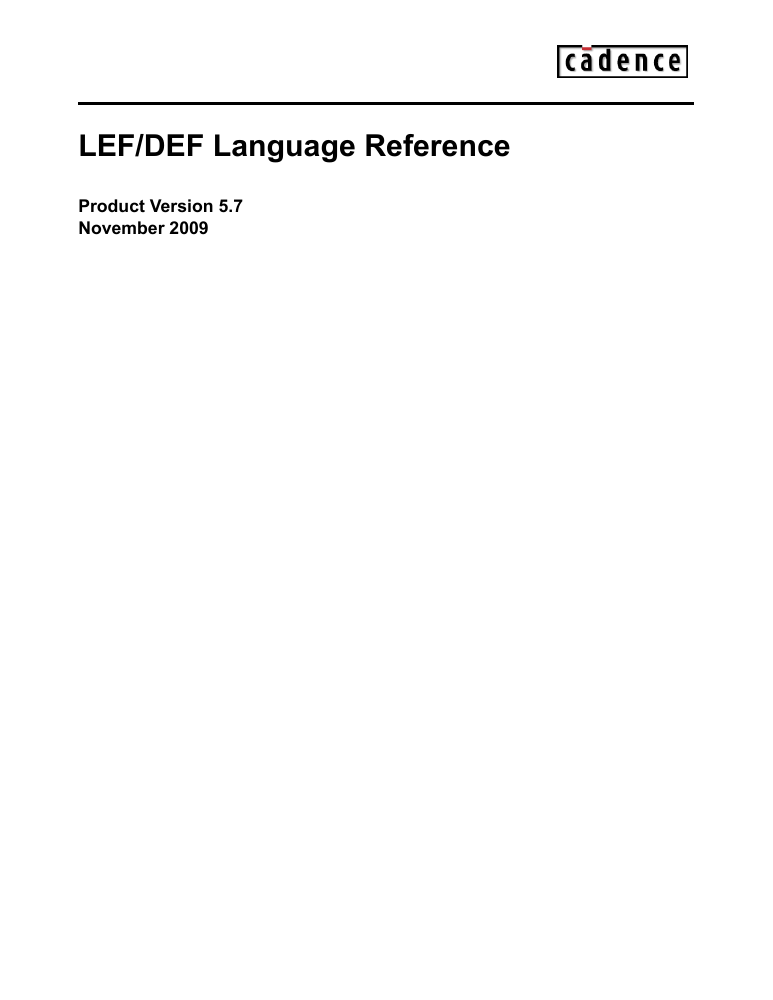
\includegraphics[height=.68\textheight]{assets/lefdef-cover.png}}
\end{column}
\begin{column}{.68\textwidth}
{\large\textcolor{NordBlue}{Cadence specification, donated to Si2}}\\[12pt]
{\textcolor{NordBlue}{LEF · Library Exchange Format}}\\[3pt]
Cell outlines and pins; technology rules\\
for placement and routing\\[13pt]
{\textcolor{NordBlue}{DEF · Design Exchange Format}}\\[3pt]
LEF's companion: physical placement of instances,\\
pins and routes --- the chip's assembled layout\\[15pt]
{\small\textcolor{NordBlue}{Reference editions}}\\[4pt]
{\small 5.6 · 2004\qquad 5.7 · 2009\qquad 5.8 · 2017}
\end{column}\end{columns}
\note{Cadence developed and released these formats for public interchange; Si2 distributes the specification and implementation. The LEF text specification was donated in 1999; DEF followed in the public offering. The format's earlier origins are Tangent Systems, acquired by Cadence in 1989. Dates shown are verified reference-manual editions, not assertions of each version's first release: 5.6 September 2004; 5.7 November 2009; 5.8 May 2017. Si2 now also lists 6.0; this short timeline selects editions relevant to these examples. Cover: Cadence LEF/DEF Language Reference 5.7, November 2009. Sources: research/SOURCES.md.}
\end{frame}
\begin{frame}{Physical view: the LEF pins}
\centering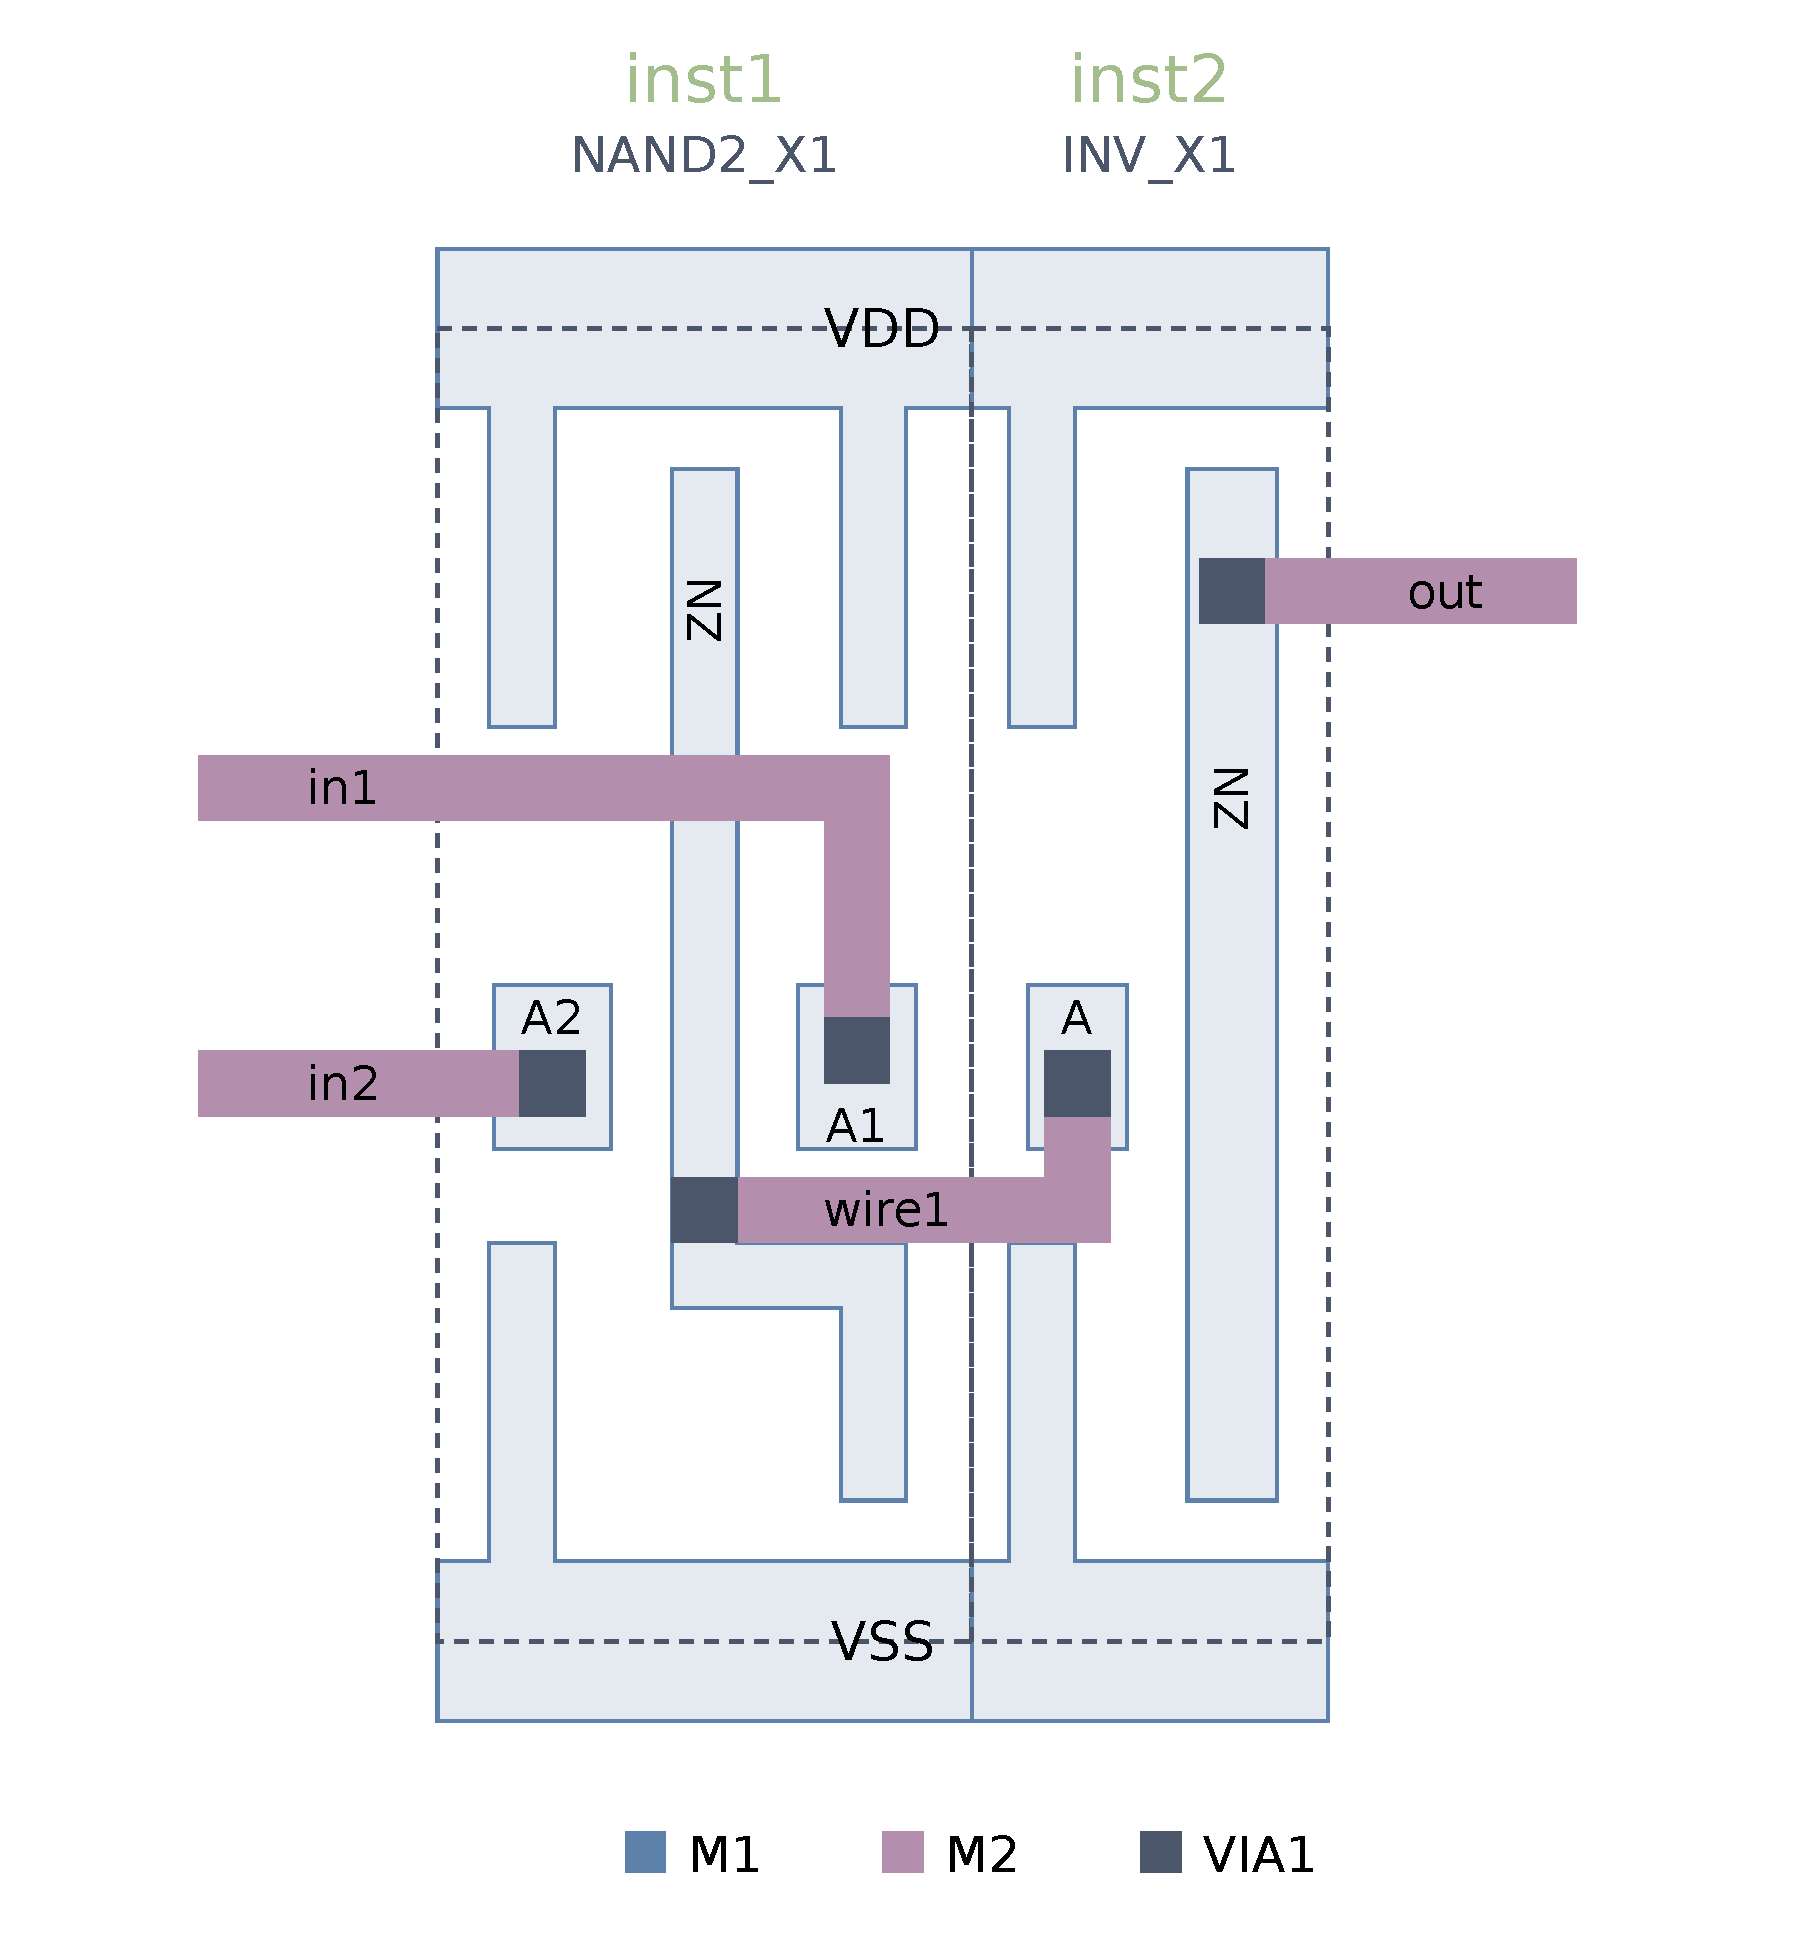
\includegraphics[height=.82\textheight]{layout/pair_pins_labeled.pdf}
\note{The cell interiors are replaced by the actual LEF PORT polygons for A1, A2, A, ZN, VDD and VSS. The same manually added M2 routes and vias are overlaid. This pin-only view omits any LEF obstructions and other technology constraints; it is not a complete router input. For these simple cells, much of M1 is exposed as pin geometry, so this looks similar to the filtered GDS view. Sources and reproduction instructions are in layout/README.md.}
\end{frame}

\begin{frame}{LEF: a master and its placement boundary}
\slidesource{\href{https://github.com/The-OpenROAD-Project/OpenROAD-flow-scripts/blob/master/flow/platforms/nangate45/lef/NangateOpenCellLibrary.macro.lef}{Cell LEF}}
\centering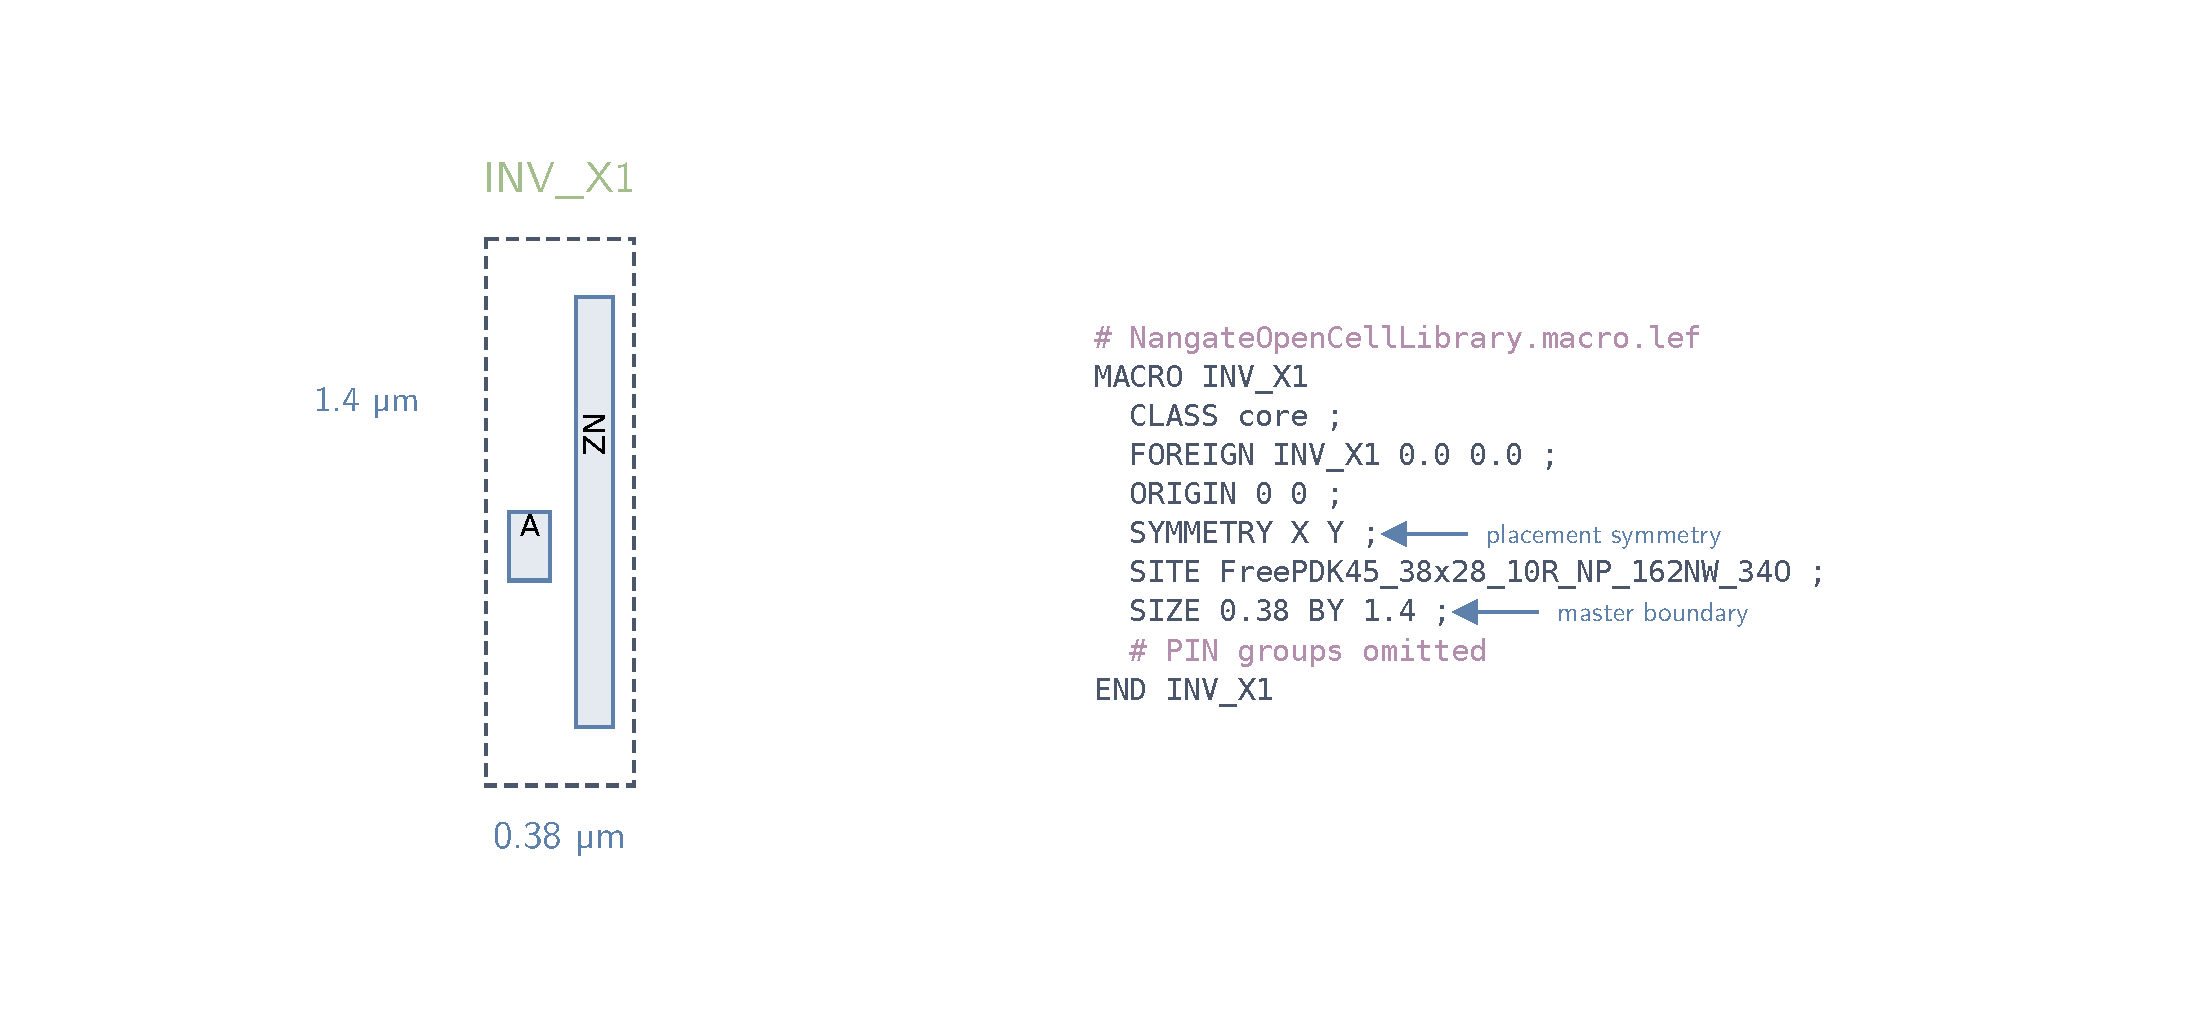
\includegraphics[width=\textwidth,height=.81\textheight,keepaspectratio]{assets/extension/lef_macro.pdf}
\note{Source excerpt retains Nangate45 values; comments mark omissions. The left diagram illustrates the highlighted quantities. Cell coordinates are in micrometers. See examples/extension for editable excerpts.}
\end{frame}

\begin{frame}{LEF: a signal pin is geometry}
\slidesource{\href{https://github.com/The-OpenROAD-Project/OpenROAD-flow-scripts/blob/master/flow/platforms/nangate45/lef/NangateOpenCellLibrary.macro.lef}{Cell LEF}}
\centering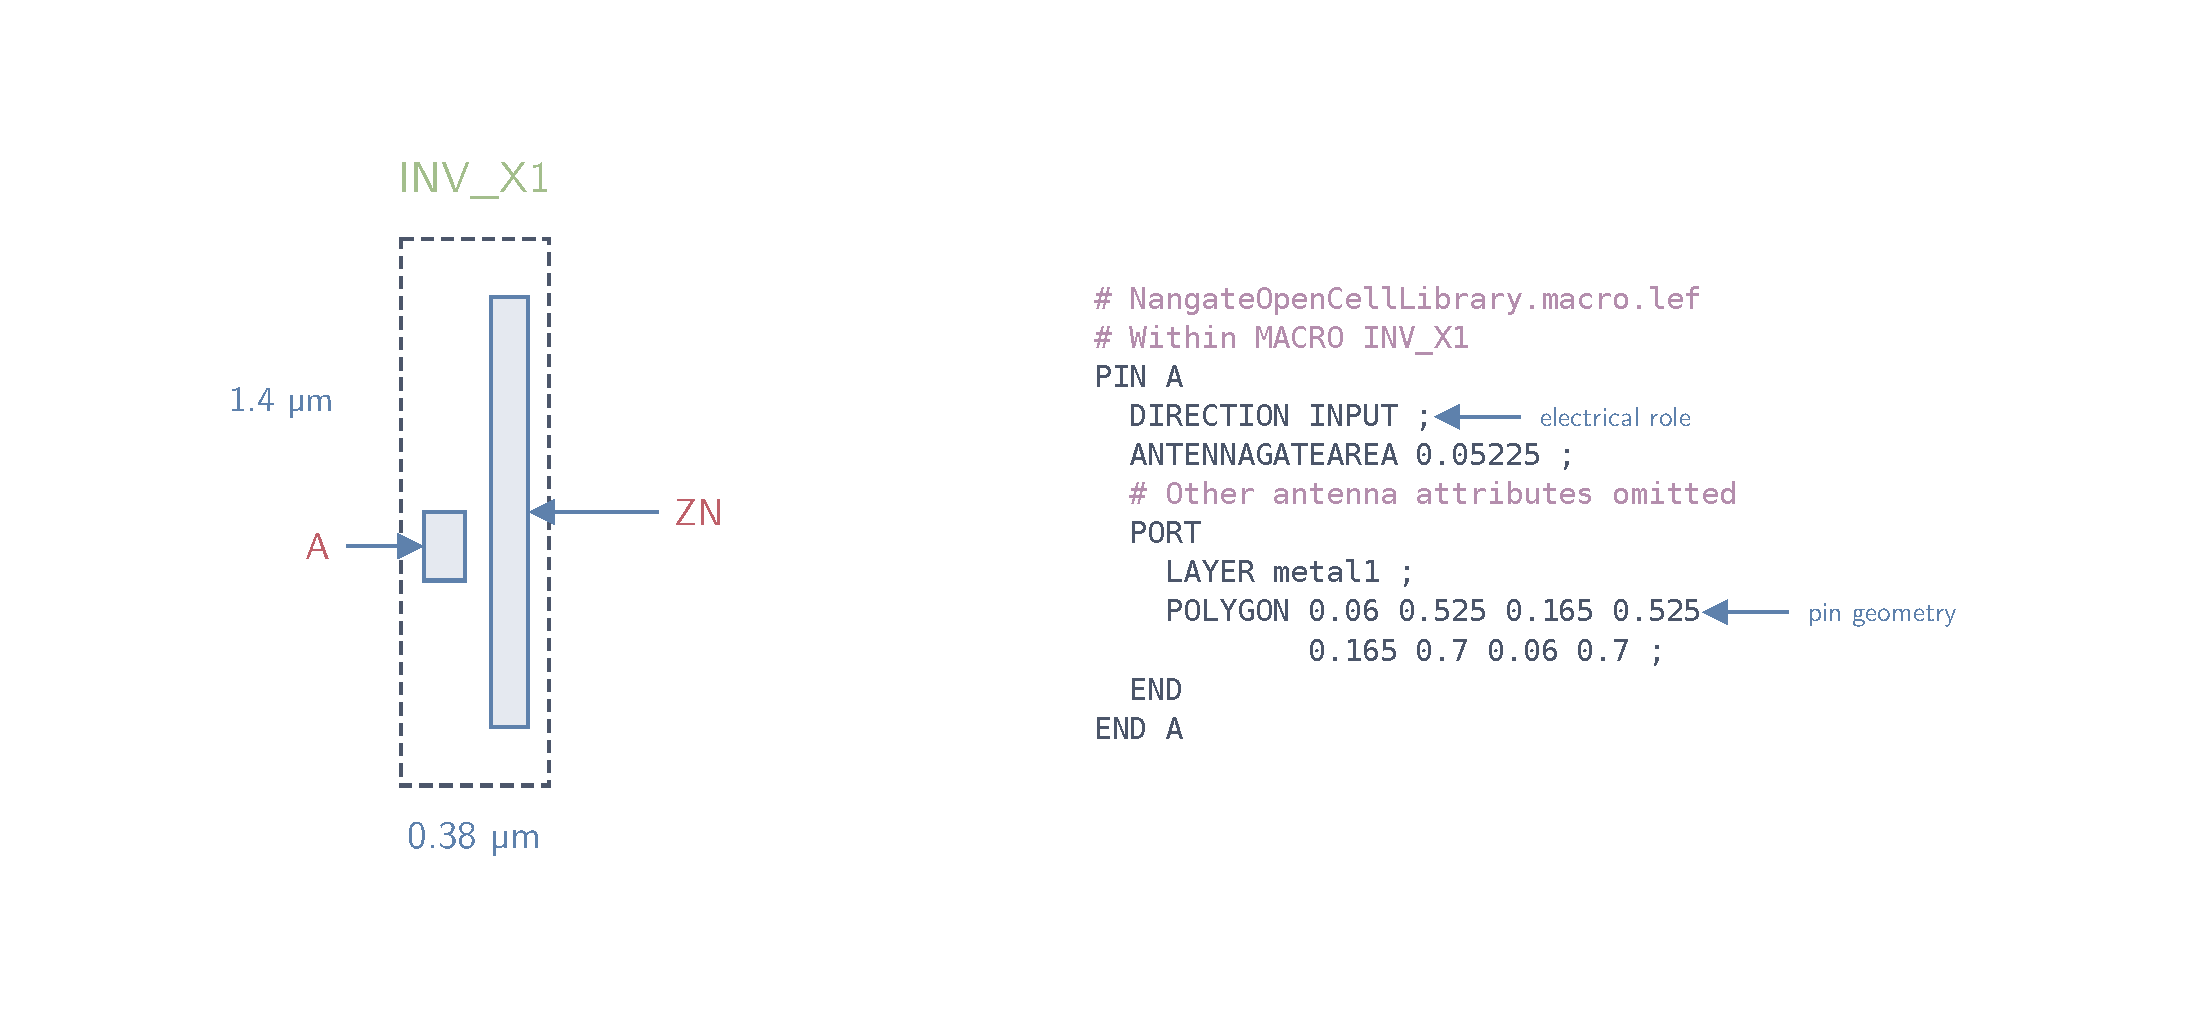
\includegraphics[width=\textwidth,height=.81\textheight,keepaspectratio]{assets/extension/lef_signal.pdf}
\note{Source excerpt retains Nangate45 values; comments mark omissions. The left diagram illustrates the highlighted quantities. Cell coordinates are in micrometers. See examples/extension for editable excerpts.}
\end{frame}

\begin{frame}{LEF: power pins and rails}
\slidesource{\href{https://github.com/The-OpenROAD-Project/OpenROAD-flow-scripts/blob/master/flow/platforms/nangate45/lef/NangateOpenCellLibrary.macro.lef}{Cell LEF}}
\centering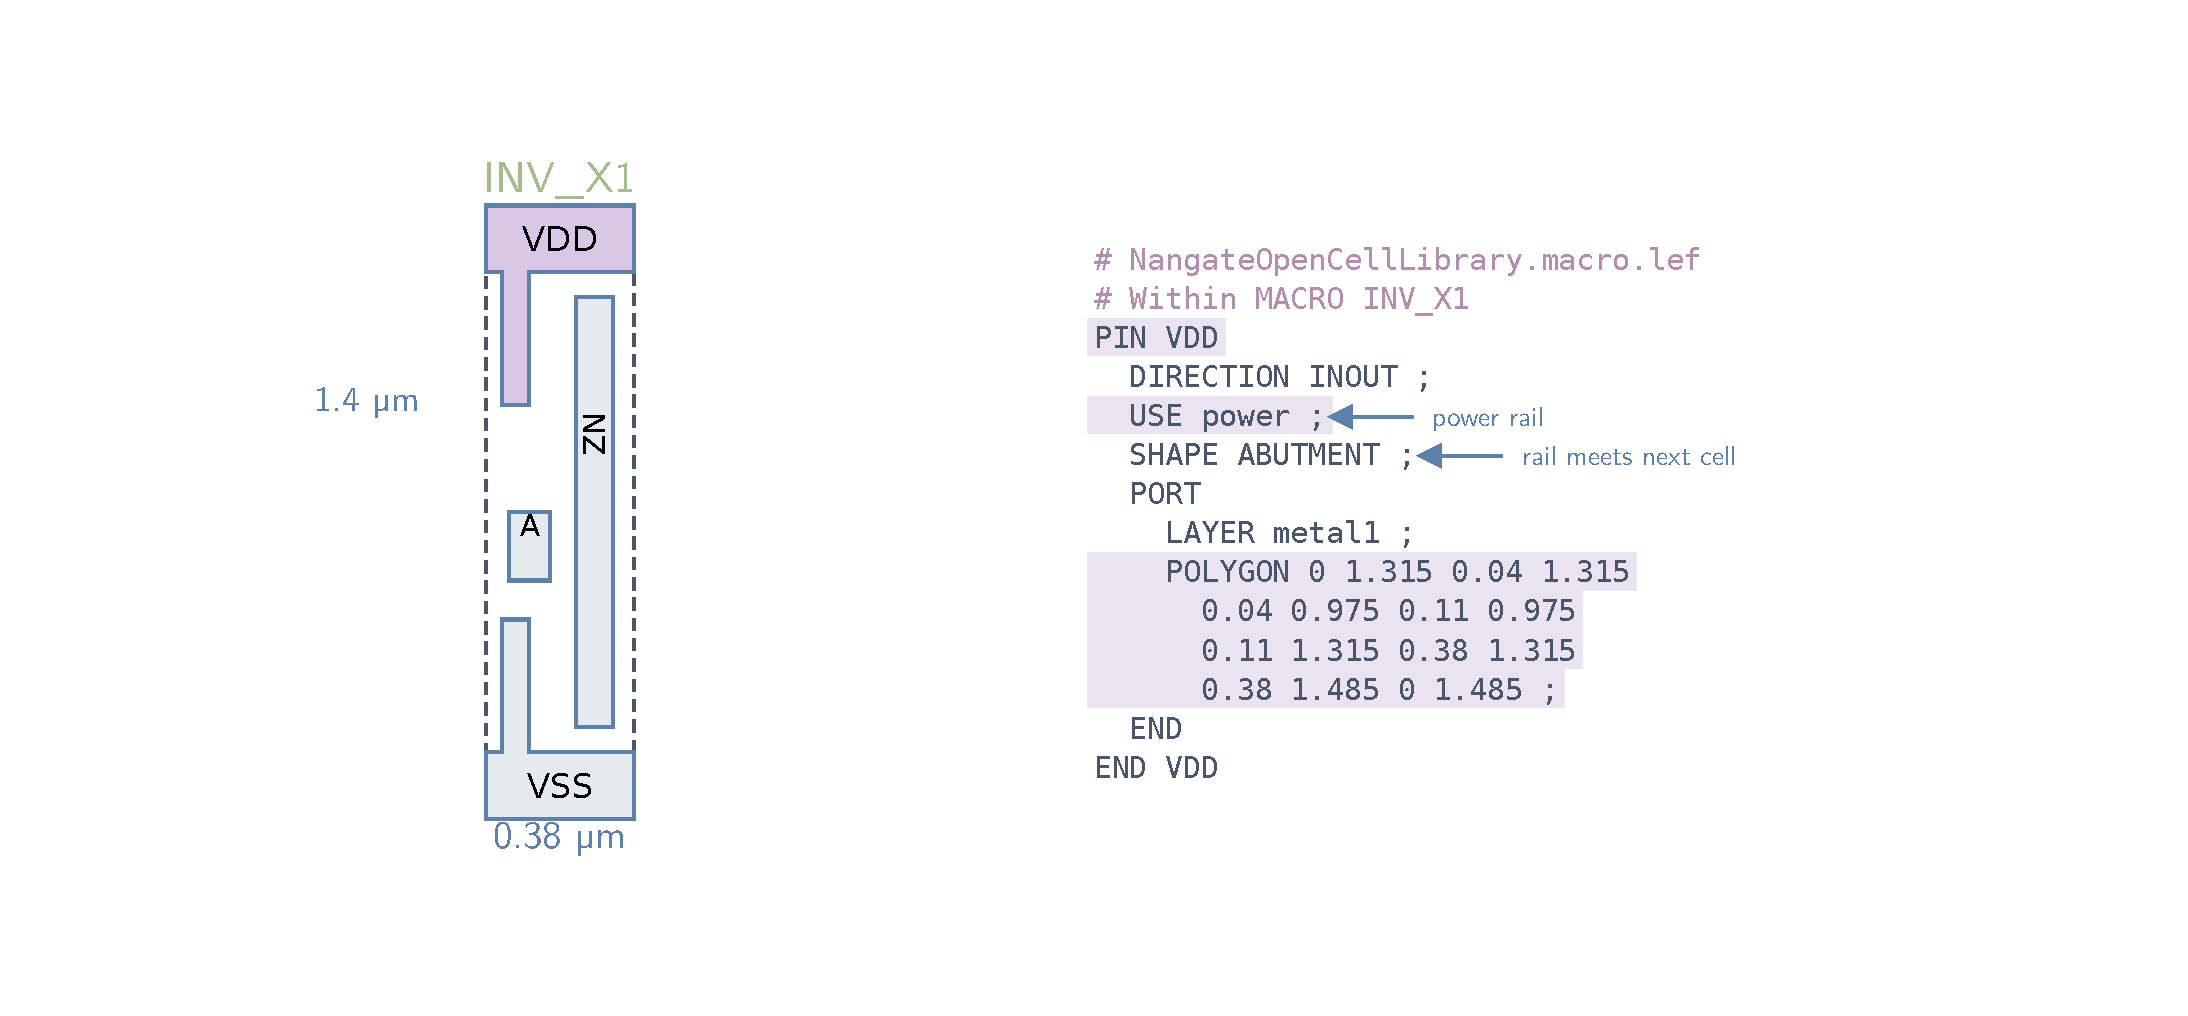
\includegraphics[width=\textwidth,height=.81\textheight,keepaspectratio]{assets/extension/lef_power.pdf}
\note{Source excerpt retains Nangate45 values; comments mark omissions. The left diagram illustrates the highlighted quantities. Cell coordinates are in micrometers. See examples/extension for editable excerpts.}
\end{frame}

\begin{frame}{LEF: units, manufacturing grid and sites}
\slidesource{\href{https://github.com/The-OpenROAD-Project/OpenROAD-flow-scripts/blob/master/flow/platforms/nangate45/lef/NangateOpenCellLibrary.tech.lef}{Tech LEF}}
\centering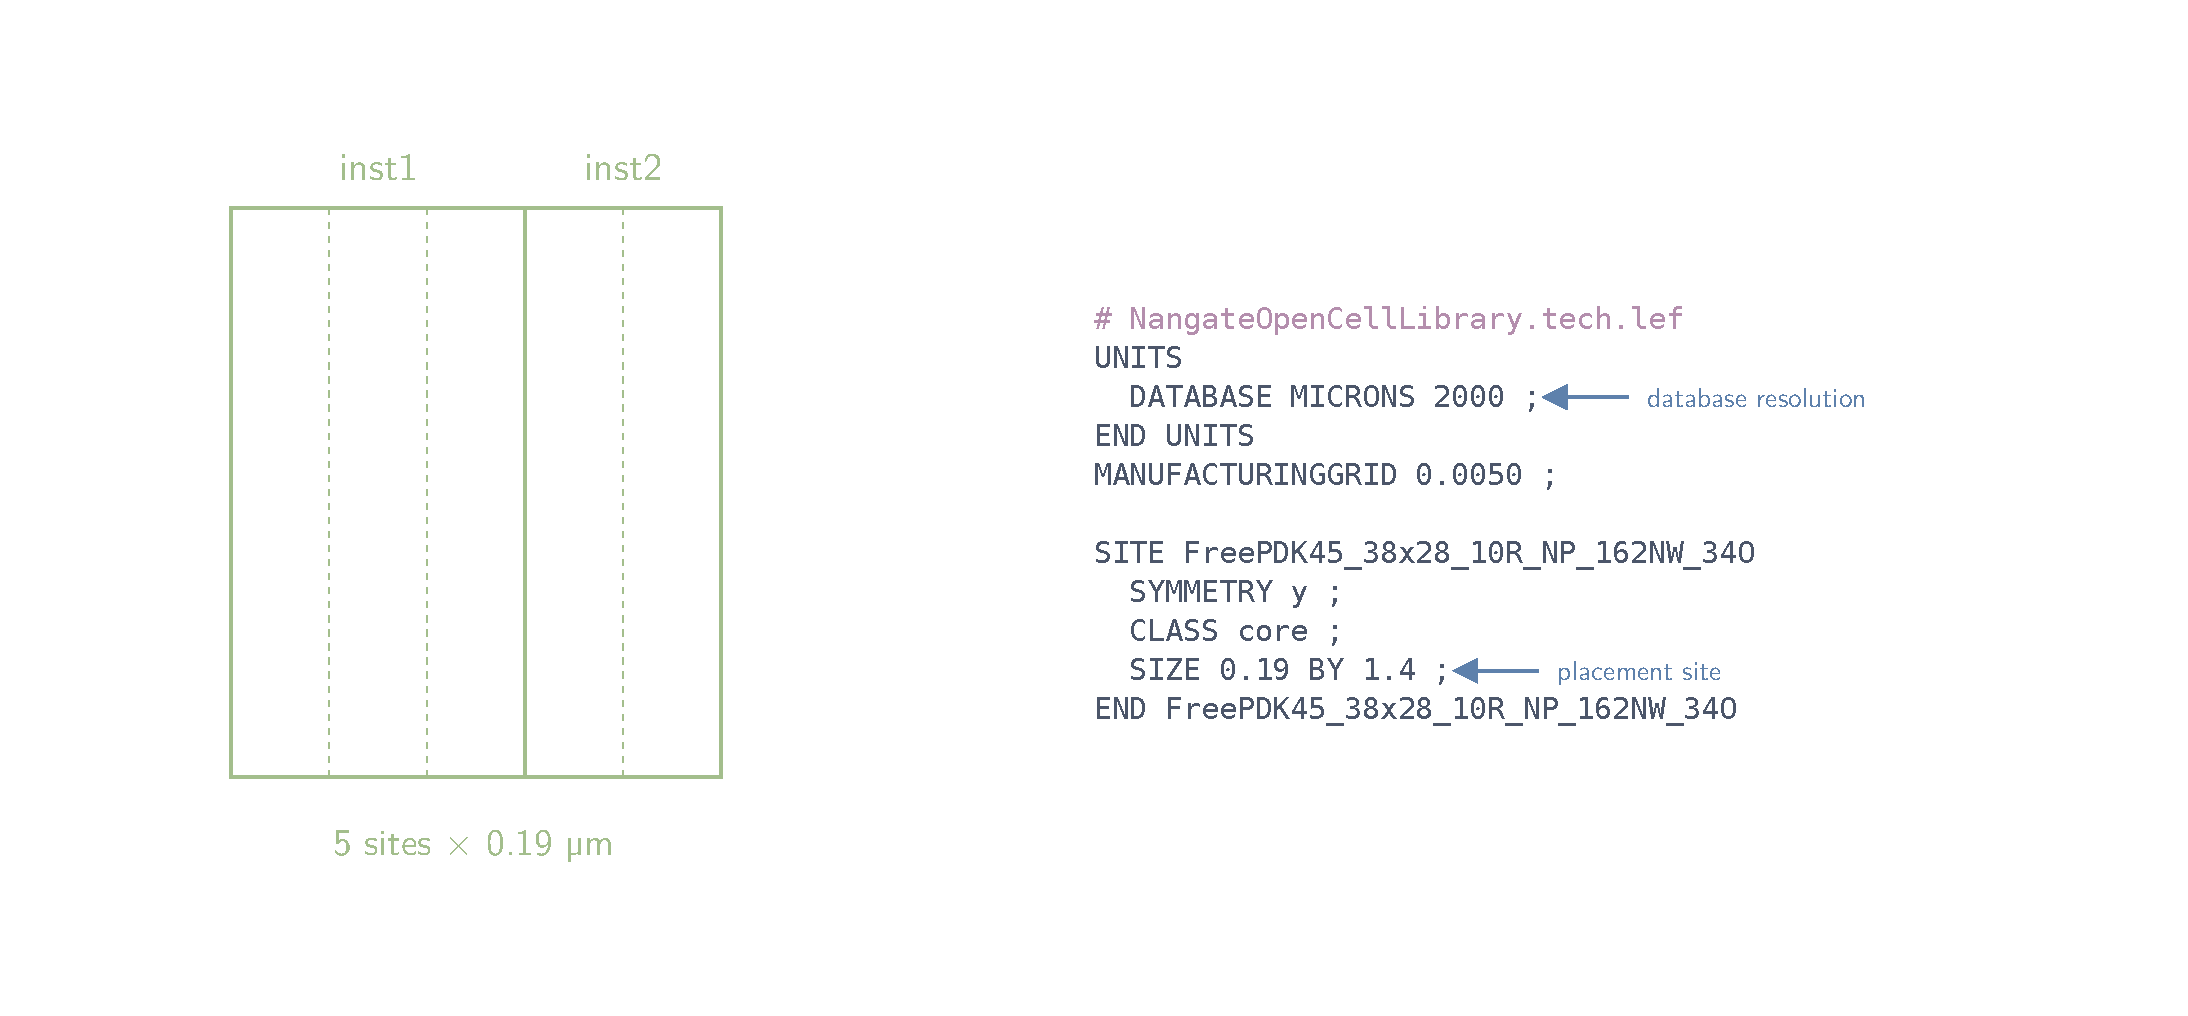
\includegraphics[width=\textwidth,height=.81\textheight,keepaspectratio]{assets/extension/lef_site.pdf}
\note{Source excerpt retains Nangate45 values; comments mark omissions. The left diagram illustrates the highlighted quantities. Cell coordinates are in micrometers. See examples/extension for editable excerpts.}
\end{frame}

\begin{frame}{LEF: a routing layer}
\slidesource{\href{https://github.com/The-OpenROAD-Project/OpenROAD-flow-scripts/blob/master/flow/platforms/nangate45/lef/NangateOpenCellLibrary.tech.lef}{Tech LEF}}
\centering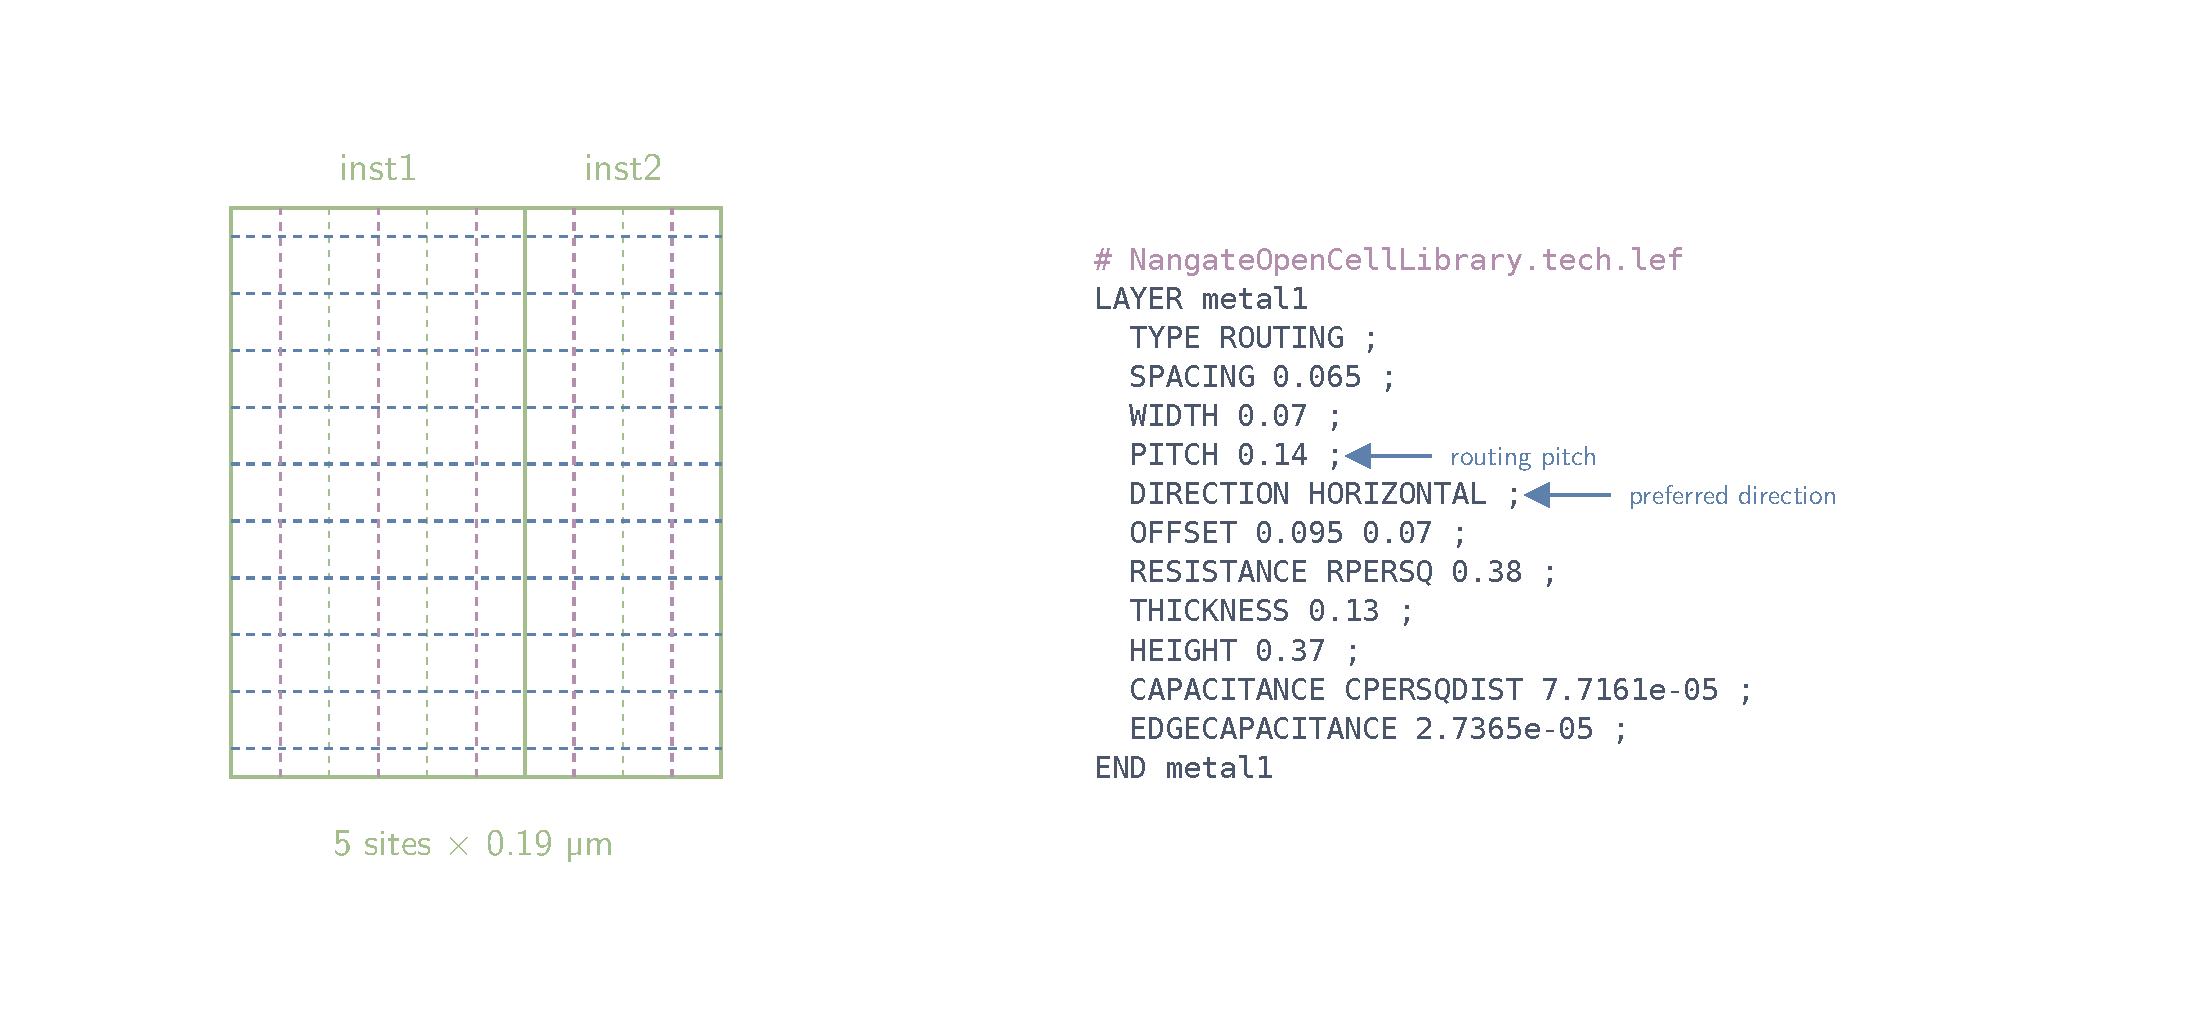
\includegraphics[width=\textwidth,height=.81\textheight,keepaspectratio]{assets/extension/lef_layer.pdf}
\note{Source excerpt retains Nangate45 values; comments mark omissions. The left diagram illustrates the highlighted quantities. Cell coordinates are in micrometers. See examples/extension for editable excerpts.}
\end{frame}

\begin{frame}{LEF: crossing between metal layers}
\slidesource{\href{https://github.com/The-OpenROAD-Project/OpenROAD-flow-scripts/blob/master/flow/platforms/nangate45/lef/NangateOpenCellLibrary.tech.lef}{Tech LEF}}
\centering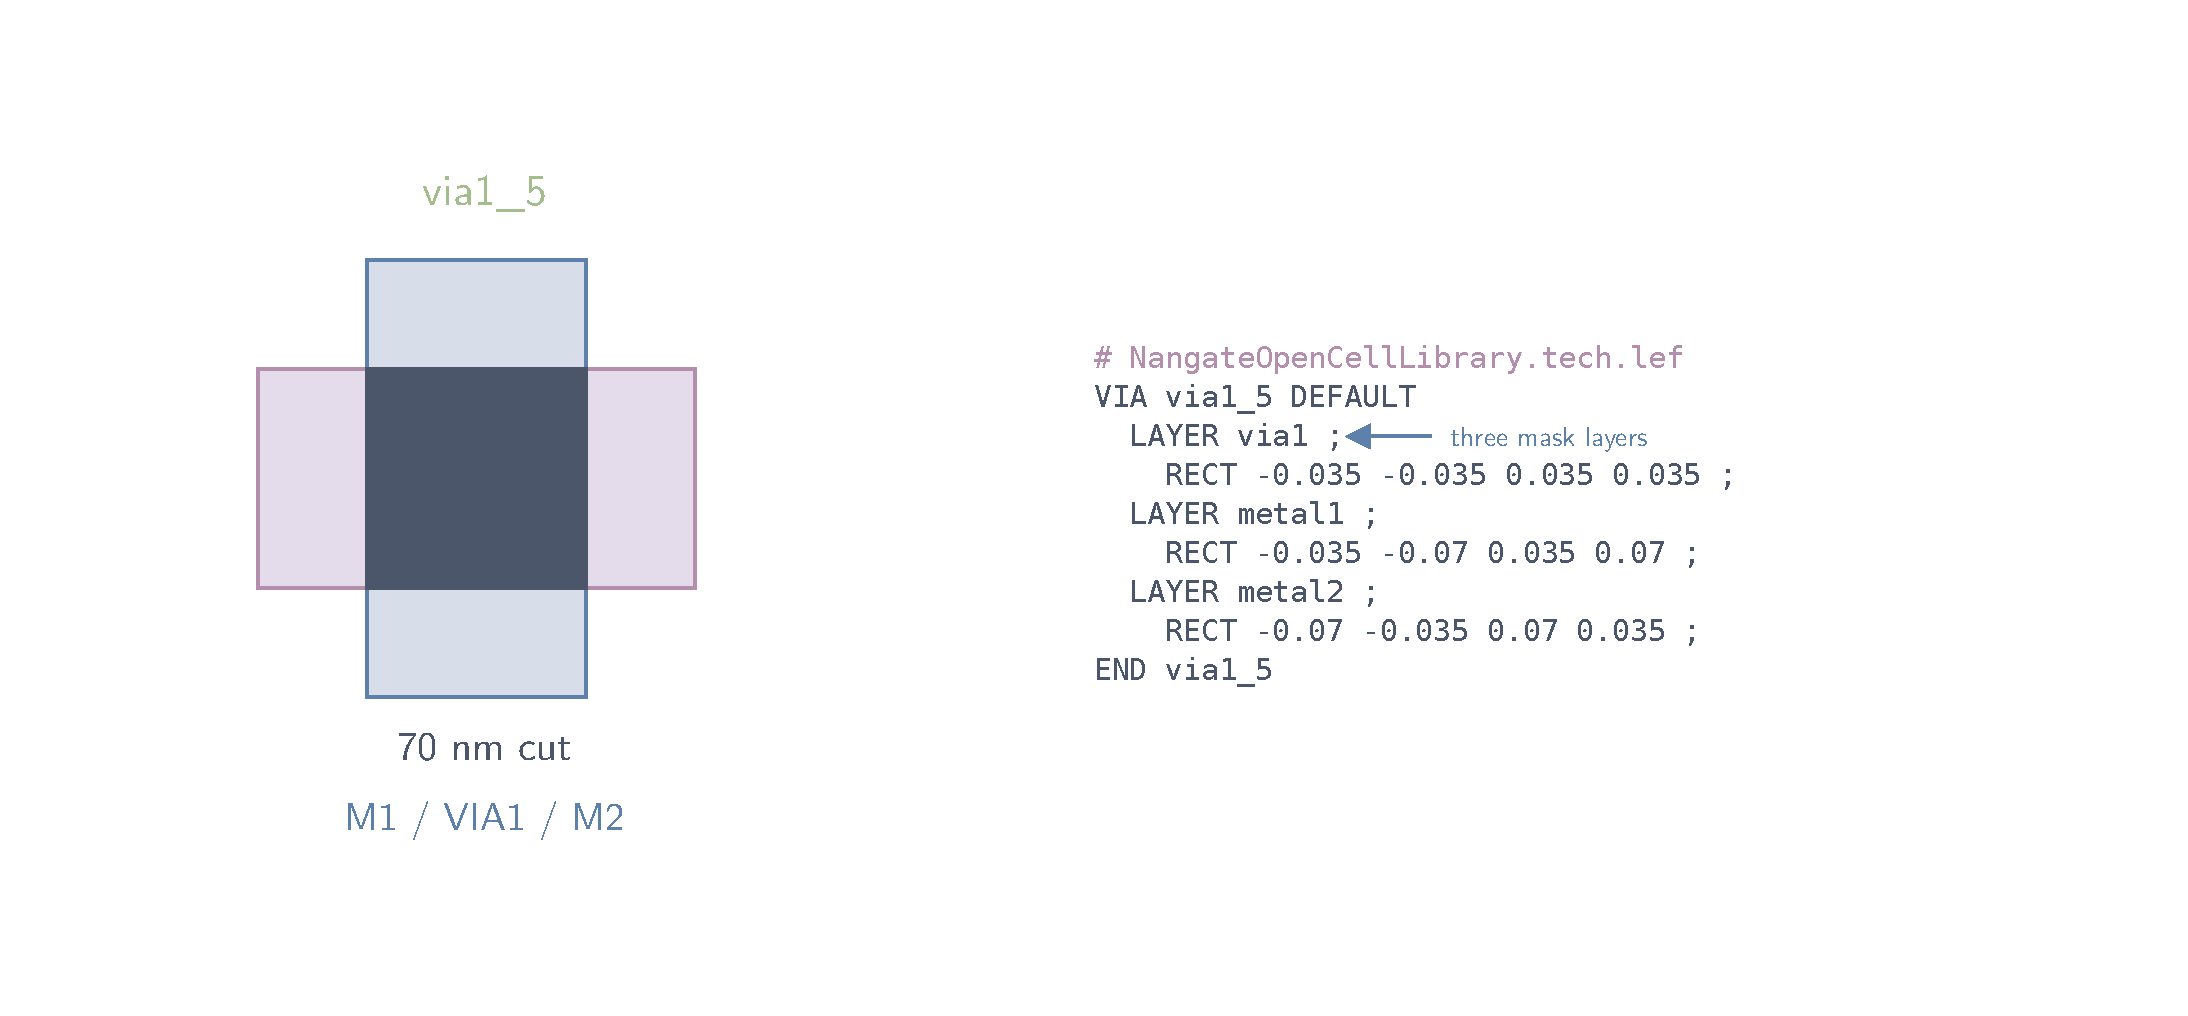
\includegraphics[width=\textwidth,height=.81\textheight,keepaspectratio]{assets/extension/lef_via.pdf}
\note{Source excerpt retains Nangate45 values; comments mark omissions. The left diagram illustrates the highlighted quantities. Cell coordinates are in micrometers. See examples/extension for editable excerpts.}
\end{frame}

\section[Timing and Power]{Timing and Power (Liberty)}

\begin{frame}{One inverter, with real input and output loading}
\slidesource{\href{https://github.com/The-OpenROAD-Project/OpenROAD-flow-scripts/blob/master/flow/platforms/nangate45/cdl/NangateOpenCellLibrary.cdl}{Cell SPICE}\enspace\textperiodcentered\enspace\href{https://ngspice.sourceforge.io/}{ngspice}}
\centering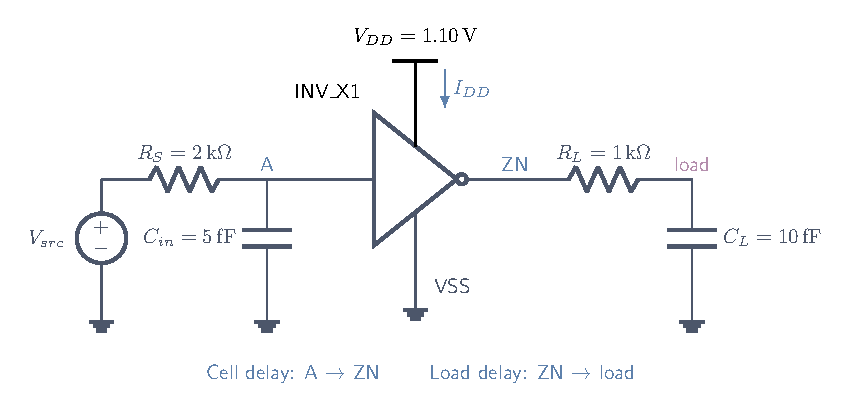
\includegraphics[width=.96\textwidth,height=.77\textheight,keepaspectratio]{assets/loaded-inverter.pdf}
\note{ngspice 45.2, real INV_X1 CDL dimensions, FreePDK45 nominal NMOS_VTL and PMOS_VTL BSIM4 cards adapted for ngspice. 1.1 V, 25 degrees C. Input 2 kilohms and 5 fF; output 1 kilohm and 10 fF. No extracted parasitics. This is an illustrative transient experiment, not reproduction of library characterization. Full executable deck: simulation/inverter_test.sp.}
\end{frame}

\begin{frame}{Propagation delay: input 50\% to output 50\%}
\slidesource{\href{https://github.com/The-OpenROAD-Project/OpenROAD-flow-scripts/blob/master/flow/platforms/nangate45/cdl/NangateOpenCellLibrary.cdl}{Cell SPICE}\enspace\textperiodcentered\enspace\href{https://ngspice.sourceforge.io/}{ngspice}}
\centering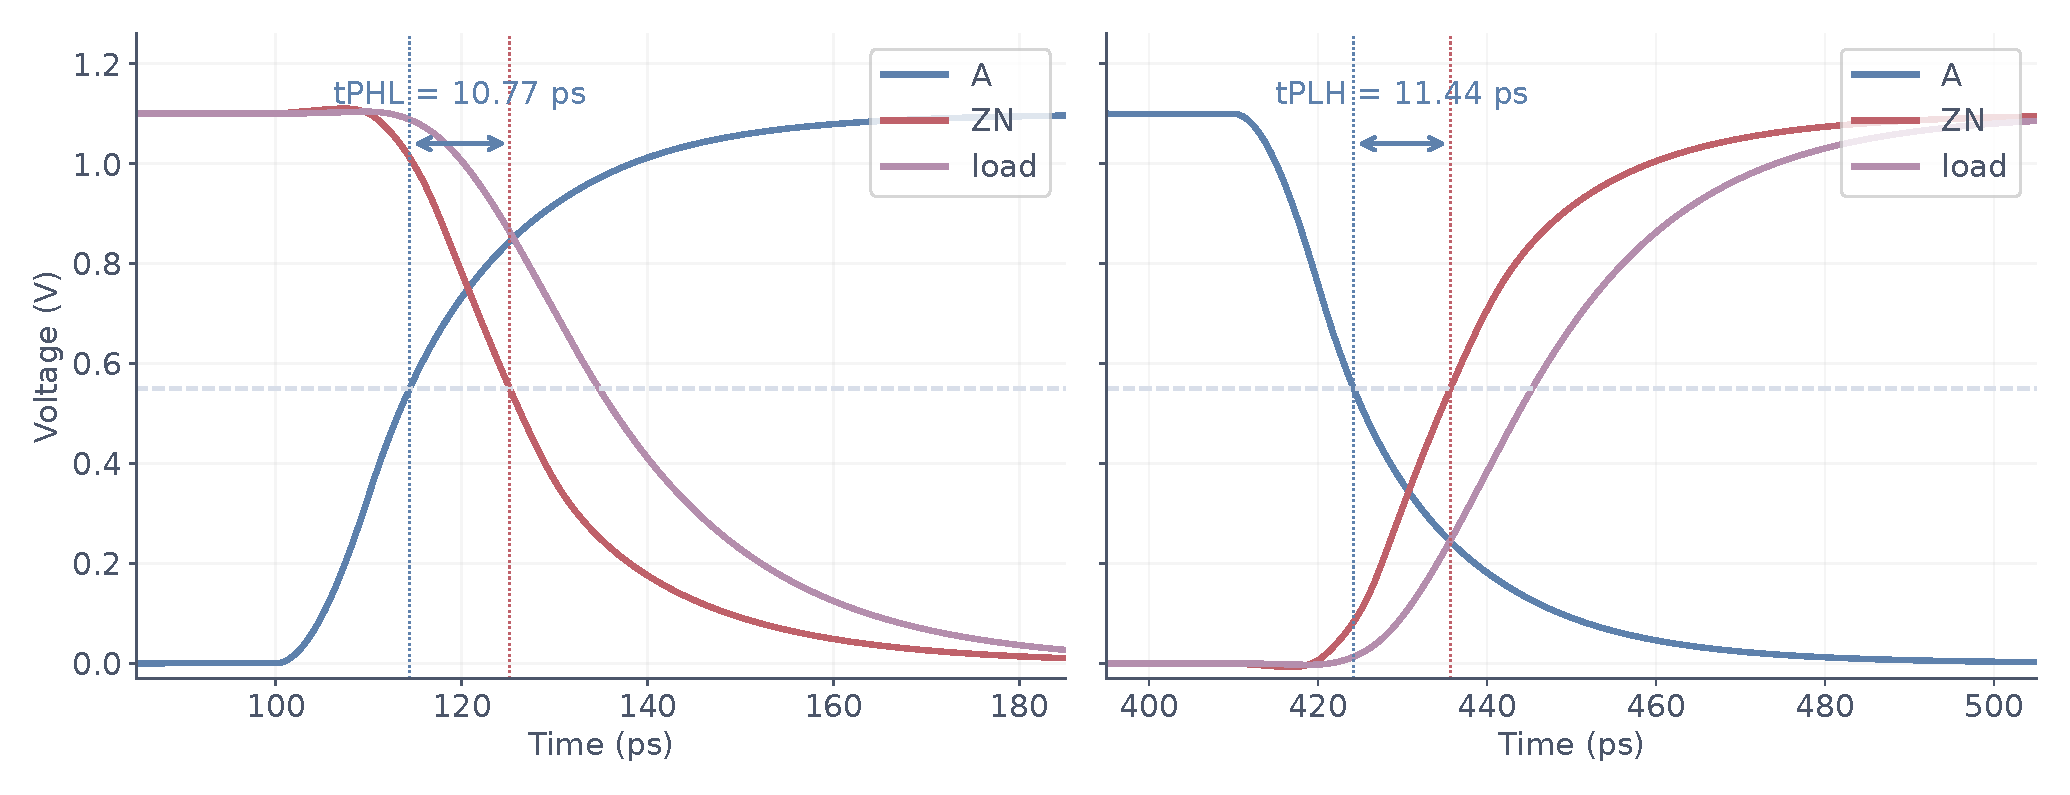
\includegraphics[width=\textwidth,height=.81\textheight,keepaspectratio]{assets/extension/propagation.pdf}
\note{Measured at cell pins A and ZN. Purple is the separate load node after the output resistor, not the cell output used for cell-delay measurement. tPHL=10.773 ps, tPLH=11.443 ps. These values depend on the chosen stimulus and RC load.}
\end{frame}

\begin{frame}{Slew: how long does the transition take?}
\slidesource{\href{https://github.com/The-OpenROAD-Project/OpenROAD-flow-scripts/blob/master/flow/platforms/nangate45/lib/NangateOpenCellLibrary_typical.lib}{Liberty}\enspace\textperiodcentered\enspace\href{https://ngspice.sourceforge.io/}{ngspice}}
\centering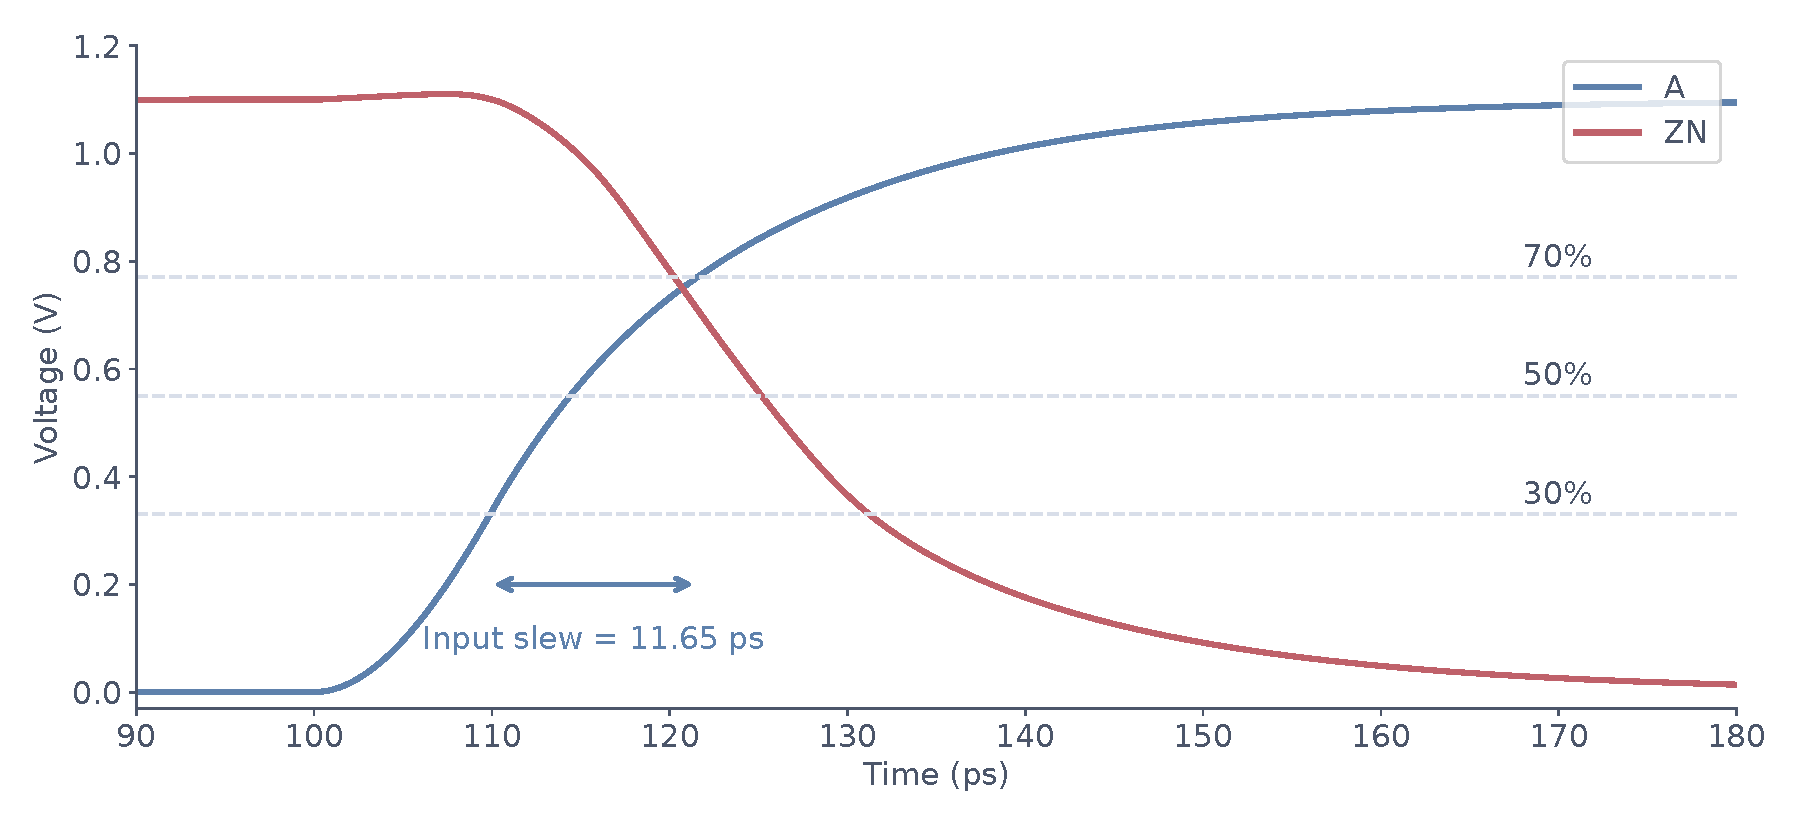
\includegraphics[width=\textwidth,height=.81\textheight,keepaspectratio]{assets/extension/slew.pdf}
\note{Nangate45 Liberty defines slew at 30 and 70 percent of the supply, and delay at 50 percent. Measured input rise slew is 11.645 ps.}
\end{frame}

\begin{frame}{Power: energy drawn from the supply}
\slidesource{\href{https://github.com/The-OpenROAD-Project/OpenROAD-flow-scripts/blob/master/flow/platforms/nangate45/cdl/NangateOpenCellLibrary.cdl}{Cell SPICE}\enspace\textperiodcentered\enspace\href{https://ngspice.sourceforge.io/}{ngspice}}
\centering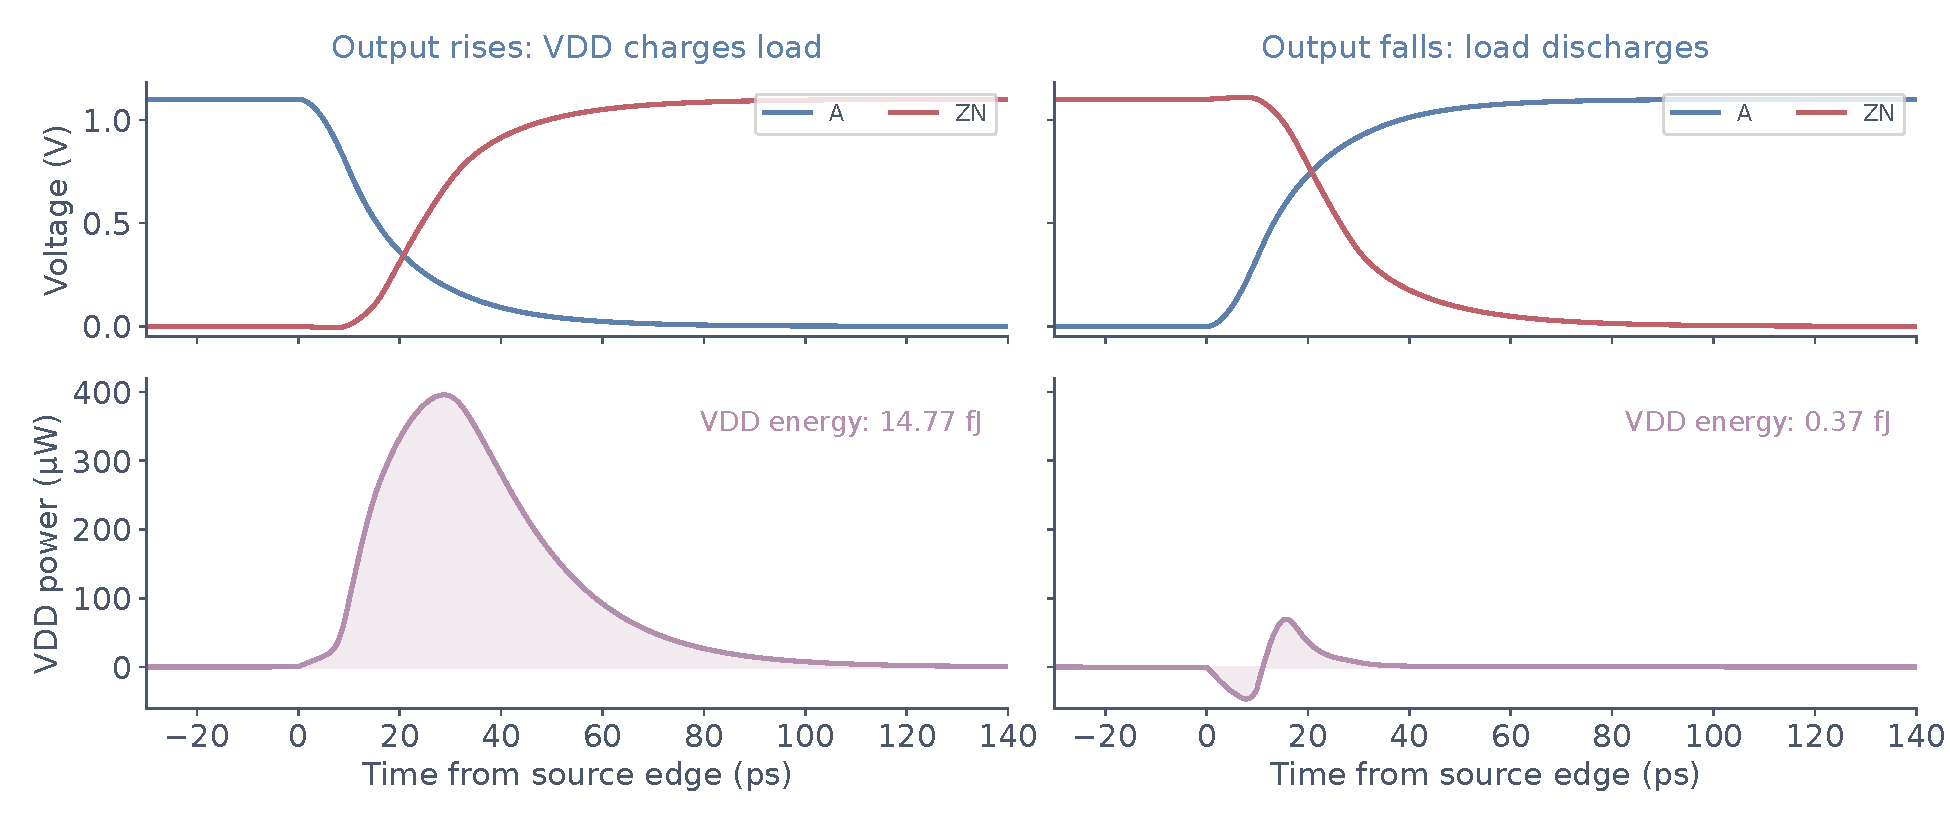
\includegraphics[width=\textwidth,height=.81\textheight,keepaspectratio]{assets/extension/power.pdf}
\note{Supply power is minus V(vdd) times current through VDD. Integral over 700 to 1400 ps is 15.136 fJ per full cycle, with our external load. The left panel shows VDD charging the load (output rising); the right panel shows output discharge (output falling). The two panels have identical scales and are aligned to their respective source edges. Energy integrates the full half-cycle windows 700--1050 ps and 1050--1400 ps: 0.370 fJ for output falling and 14.766 fJ for output rising. VDD charges the capacitor during the output rise; during output fall the stored capacitor energy is released through the pull-down network. Supply power is not the same as instantaneous heat dissipated in the devices. Brief negative power indicates energy returned to the ideal supply. It includes load charging, internal switching and leakage; it is not the Liberty internal_power value. Dynamic power depends on activity and frequency.}
\end{frame}

\begin{frame}{Liberty: characterize the cell once}
\slidesource{\href{https://en.wikipedia.org/wiki/Standard_cell}{Wikipedia}\enspace\textperiodcentered\enspace\href{https://github.com/The-OpenROAD-Project/OpenROAD-flow-scripts/blob/master/flow/platforms/nangate45/lib/NangateOpenCellLibrary_typical.lib}{Liberty}}
\begin{columns}[c,onlytextwidth]\begin{column}{.48\textwidth}\centering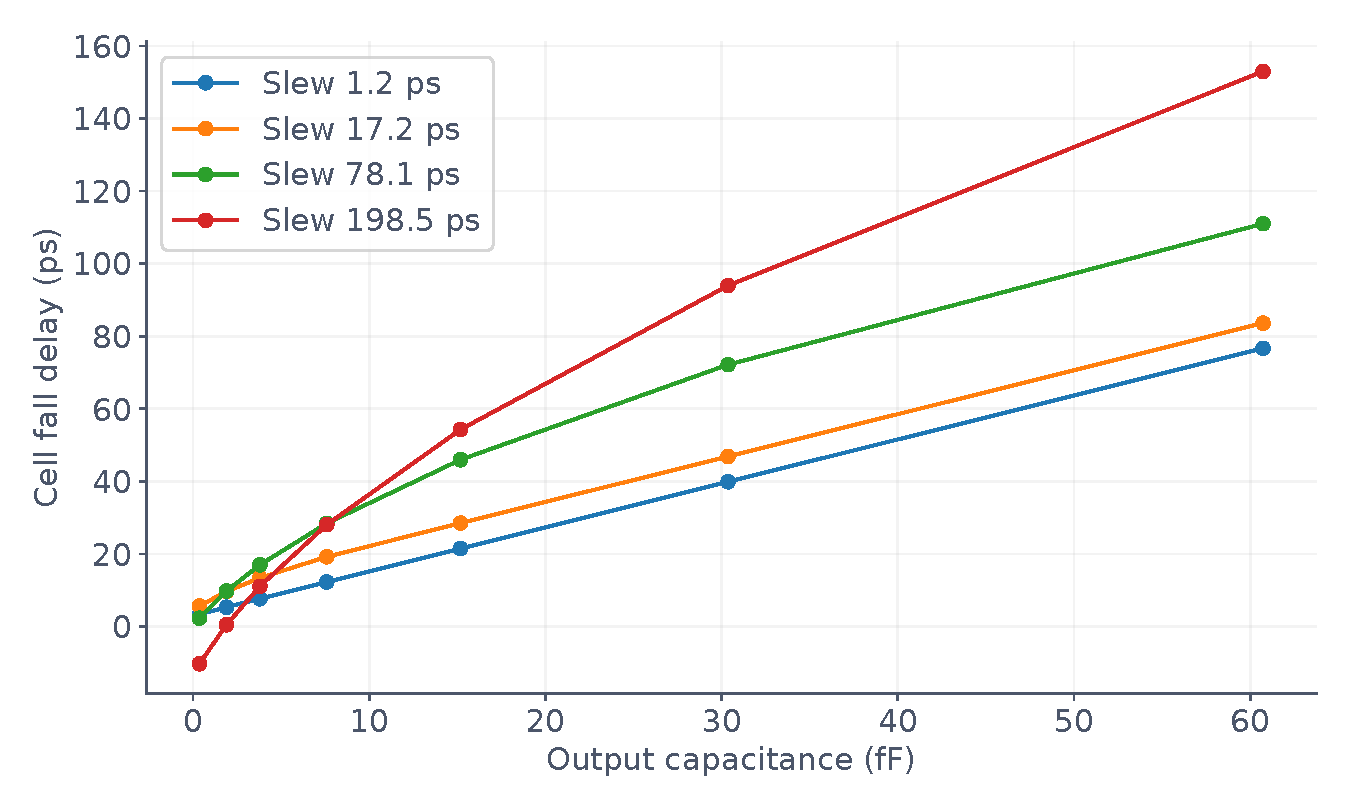
\includegraphics[width=\linewidth,height=.73\textheight,keepaspectratio]{assets/extension/liberty_table.pdf}\end{column}\begin{column}{.48\textwidth}
{\Large\textcolor{NordBlue}{Liberty (.lib)}}\\[16pt]Developed by Synopsys\\An industry library standard\\[20pt]{\large Logic, timing and power for analysis tools}\end{column}\end{columns}
\note{Liberty is a name, not an expanded acronym. Wikipedia has no dedicated Liberty-format article; the link is the related standard-cell page. Primary specification publisher: Synopsys. Plot is the actual Nangate45 INV_X1 cell_fall table, not the preceding transient experiment.}
\end{frame}

\begin{frame}{Three generations of Liberty files}
\slidesource{\href{https://www.synopsys.com/blogs/chip-design/library-characterization-for-advanced-process-designs.html}{Liberty models}}
\begin{columns}[T,onlytextwidth]
\begin{column}{.31\textwidth}
{\large\textcolor{NordBlue}{\underline{NLDM}}}\\[12pt]
\begin{itemize}\setlength{\itemsep}{7pt}
\item Simplest model: what we just showed
\item Delay and slew tables
\item Indexed by input slew and output load
\end{itemize}\vspace{10pt}
{\ttfamily\footnotesize cell\_rise / cell\_fall}
\end{column}
\begin{column}{.31\textwidth}
{\large\textcolor{NordBlue}{\underline{CCS / ECSM}}}\\[12pt]
\begin{itemize}\setlength{\itemsep}{7pt}
\item Current-waveform models
\item Capture waveform shape and load response
\item More detailed nominal timing
\end{itemize}\vspace{10pt}
{\ttfamily\footnotesize output\_current\_rise\\output\_current\_fall}
\end{column}
\begin{column}{.31\textwidth}
{\large\textcolor{NordBlue}{\underline{LVF}}}\\[12pt]
\begin{itemize}\setlength{\itemsep}{7pt}
\item Statistical variation data
\item Describe variation in delay and slew
\item Add to nominal timing models
\end{itemize}\vspace{10pt}
{\ttfamily\footnotesize ocv\_sigma\_cell\_rise\\ocv\_sigma\_cell\_fall}
\end{column}
\end{columns}
\note{Generations is used as a teaching shorthand for the evolution of library modeling, not mutually exclusive file-format versions. A Liberty file can contain NLDM tables, current-source models such as CCS, and LVF variation data. CCS/ECSM provide richer nominal behavior; LVF describes statistical variation rather than simply replacing the nominal model with a more accurate one. output_current_rise/fall are CCS keywords, not generic ECSM syntax. The Nangate45 example uses NLDM.}
\end{frame}

\end{document}
